% Preamble
\documentclass{article}


% Packages
\usepackage{../../../mypackages}


% Macros
\usepackage{../../../mymacros}


% File Info
\title{PHYS141 Notes}
\author{Eric Xia}
\date{Last Updated 27 December 2020}


% Document
\begin{document}

    \maketitle
    \tableofcontents
    \pagebreak


    \section{Introduction}

    \textbf{Rational:} maximally achieving pre-defined goals; maximizing your expected utility \\
    \textbf{Rationality}: only concerns what decisions are made and not the thought process behind them \\

    Artificial intelligence is often observed in two dimensions, human vs. rational and thought (internal reasoning) vs. behavior (external characterization) \\

    \textbf{Turing Test:} designed as a thought experiment to sidestep the philosophical vagueness of the question "can a machine think?", would need the following capabilities: \\
    $\bullet$ \textbf{Natural language processing} to communicate successfully in a human language \\
    $\bullet$ \textbf{Knowledge representation} to store what it knows or hears \\
    $\bullet$ \textbf{Automated reasoning} to answer questions and to draw new conclusions \\
    $\bullet$ \textbf{Machine learning} to adapt to new circumstances and to detect and extrapolate patterns \\

    \textbf{Total Turing Test:} requires interaction with objects and people in the real world, proposed because Turing viewed the \textit{physical} simulation of a person as unnecessary to demonstrate intelligence,
    the robot would need: \\
    $\bullet$ \textbf{Computer vision:} and speech recognition to perceive the world \\
    $\bullet$ \textbf{Robotics} to manipulate objects and move about \\
    \textbf{Agent:} an entity that operates autonomously, perceives its environment, persists over a prolonged time period, adapts to change, and creates and pursues goals \\
    \textbf{Rational agent:} selects actions that maximize its (expected) utility \\
    \textbf{Limited rationality:} acting appropriately when there is not enough time to do all the computations one might like \\
    \textbf{Value alignment problem:} the values or objectives put into the machine must be aligned with those of the human \\
    \textbf{Incompleteness theorem:} in any formal theory as strong as Peano arithmetic (the elementary theory of natural numbers), there are necessarily true statements that have no proof within the theory \\
    \textbf{Computability:} capable of being computed by an effective procedure \\
    \textbf{Tractability:} a problem is intractable if the time required to solve instances of the problem grows exponentially with the size of the instances \\
    \textbf{NP-completeness:} provides a basis for analyzing the tractability of problems: any problem class to which the class of NP-complete problems can be reduced is likely to be intractable \\
    \textbf{Decision theory:} combines probability theory with utility theory and provides a formal and complete framework for individual decisions made under uncertainty \\
    \textbf{Satisficing:} making decisions that are "good enough" rather than laboriously calculating an exact optimal decision \\


    \section{Foundations}

    \subsection{Representations}

        Visual representations are a vital part of understanding a problem and developing a model. Reprsentations may include pictures, sketches, diagrams, graphs, and a multitude of context-specific procedures.
        To avoid cluttering a reprsentation, it is best to oversimplify a real-life situation and gradually construct less idealized models. It our oversimplified model reproduces the main features of its real-world
        counterpart, then we know we have chosen adequate essential attributes. \\

        \noindent In this respect, mathematical symbols also act as representations of more complex phrases. Take, for example, the statement below.

        \begin{quote}
            "The magnitude of the acceleration of an object is directly proportional to the magnitude of the vector sum of the forces exerted on the object and inversely proportional to the object's inertia.
            The direction of the acceleration is the same as the direction of the vector sum of the forces."
        \end{quote}

        \noindent This can be expressed concisely and more clearly with the mathematic equation,

        \begin{equation*}
            \overrightarrow{a} = \frac{\sum \overrightarrow{F}}{m}
        \end{equation*}


    \subsection{Physical quantities and units}

        \textbf{Physical quantities and their symbols}:

        \begin{center}
            \begin{tabular}{|c|c|}
                \hline
                \textbf{Physical Quantity}  & \textbf{Symbol} \\
                \hline
                length                      & $l$ \\
                \hline
                time                        & $t$ \\
                \hline
                mass                        & $m$ \\
                \hline
                speed                       & $v$ \\
                \hline
                volume                      & $V$ \\
                \hline
                energy                      & $E$ \\
                \hline
                temperature                 & $T$ \\
                \hline
            \end{tabular}
        \end{center}

        \noindent Physical quantities are expressed as the product of a number and a unit of measurement. For example, the length $l$ of an object that is $1.2 m$ long can be expressed as $l=1.2m$. The global unit system
        used in science and engineering is the \textbf{Syst\'eme International (SI)}. There are seven base units in the SI system from which all other units can be derived. \\

        \noindent \textbf{The Seven SI Base Units:}

        \begin{center}
            \begin{tabular}{|c|c|c|}
                \hline
                \textbf{Name of Unit}   & \textbf{Abbreviation} & \textbf{Physical Quantity} \\
                \hline
                meter                   & m                     & length \\
                \hline
                kilogram                & kg                    & mass \\
                \hline
                second                  & s                     & time \\
                \hline
                ampere                  & A                     & electric current \\
                \hline
                kelvin                  & K                     & thermodynamic temperature \\
                \hline
                mole                    & mol                   & amount of substance \\
                \hline
                candela                 & cd                    & luminous intensity \\
                \hline
            \end{tabular}
        \end{center}

        \noindent To work conveniently with very large or very small numbers, we modify the unit name with prefixes representing integer powers of ten, conventionally powers of ten that are multiples of 3. For example,
        a billionth of a second is denoted by 1 ns and pronounced "one nanosecond", where 1 ns $=$ $10^{-9}$s. \\

        \noindent \textbf{SI Prefixes:}

        \begin{center}
            \begin{tabular}{|c|c|c|}
                \hline
                $\bm{10^n}$ & \textbf{Prefix}   & \textbf{Abbreviation} \\
                \hline
                $10^{24}$   & yotta-            & Y \\
                \hline
                $10^{21}$   & zetta-            & Z \\
                \hline
                $10^{18}$   & exa-              & E \\
                \hline
                $10^{15}$   & peta-             & P \\
                \hline
                $10^{12}$   & tera-             & T \\
                \hline
                $10^9$      & giga-             & G \\
                \hline
                $10^6$      & mega-             & M \\
                \hline
                $10^3$      & kilo-             & k \\
                \hline
                $10^0$      & \sout{     }      & \sout{  } \\
                \hline
                $10^{-3}$   & milli-            & m \\
                \hline
                $10^{-6}$   & micro-            & $\mu$ \\
                \hline
                $10^{-9}$   & nano-             & n \\
                \hline
                $10^{-12}$  & pico-             & p \\
                \hline
                $10^{-15}$  & femto-            & f \\
                \hline
                $10^{-18}$  & atto-             & a \\
                \hline
                $10^{-21}$  & zepto-            & z \\
                \hline
                $10^{-24}$  & yocto-            & y \\
                \hline
            \end{tabular}
        \end{center}

        \noindent A \textbf{mole} is currently defined as the number of atoms in $12\times 10^{-3}$ kg of carbon-12. This number is referred to as \textbf{Avogrado's number ($N_A$)}, where the currently accepted
        measurement of Avogradro's number is

        \begin{equation*}
            N_A = 6.0221413 \times 10^{23}
        \end{equation*}

        \noindent \textbf{Density} is the physical quantity measuring how much of some substance exists in a given volume. \textbf{Number density} is the number of objects per unit volume. If there are $N$ objects in a
        volume $V$, then the number density $n$ of these objects is

        \begin{tbhtheorem}{Number Density}
            $n = \frac{N}{V}$
        \end{tbhtheorem}

        \noindent \textbf{Mass density ($\rho$)} is the amount of mass $m$ per unit volume:

        \begin{tbhtheorem}{Mass Density}
            $\rho = \frac{m}{V}$
        \end{tbhtheorem}

        \noindent The easiest way to convert measurements to other units is to write the \textbf{conversion factor} as a fraction. Then multiply what you're to express by the conversion ratio, cancelling out the units.
        Below is an example of converting 4.5 inches to millimeters:

        \begin{equation*}
            4.5 \text{ in. } = (4.5 \cancel{\text{ in. }})\left(\frac{25.4\text{ mm}}{1 \cancel{\text{ in.}}}\right) = 4.5 \times 25.4 \text{ mm } = 1.1 \times 10^2 \text{ mm}
        \end{equation*}


    \subsection{From Reality to Model}

        If the position of an object is not changing, it is said to be \textbf{at rest}. A \textbf{Position-Time Graph} describes the position of an object as a function of a unit of time. Below is a position-time graph
        for walking.

        \begin{center}
            \begin{tikzpicture}[scale= ]
                \begin{axis}[
                    axis lines = center,
                    axis equal image,
                    xlabel = {Distance from origin (mm)},
                    ylabel = {Seconds},
                    xlabel near ticks,
                    ylabel near ticks,
                    xmin = 0,
                    xmax = 20,
                    ymin = 0,
                    ymax = 15,
                    xtick = {0,5,10,15,20},
                    xticklabels = {0,5,10,15,20},
                    ytick = {5,10,15},
                    yticklabels = {5,10,15}
                ]
                \draw[blue](1,2.5) -- (7.5,12.5);
                \draw[red](7.5,12.5) -- (12.5,12.5);
                \draw[ForestGreen](12.5,12.5) -- (19,8);
                \end{axis}
            \end{tikzpicture}
        \end{center}

        \noindent Here, the blue section of the graph describes when the person is walking forwards, the red section is when the person is pausing, and the green section is when the person is walking backwards.
    \section{Motion in One Dimension and Changes in Velocity}

    \subsection{Position and Displacement}
        \textbf{Position-versus-time graph}: a graph that represents position ($x$) as a function of time ($t$).

        \begin{center}
            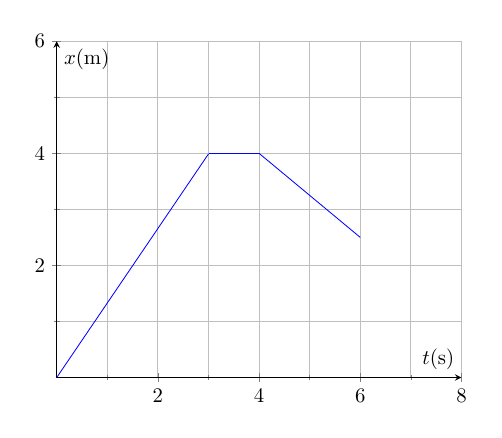
\begin{tikzpicture}[scale=0.75]
                \begin{axis}[
                    axis lines = middle,
                    smooth,
                    xlabel = $t$(s),
                    ylabel =$x$(m),
                    minor tick num =1,
                    grid=both,
                    no markers,
                    domain=0:8,
                    xtick={0,2,4,6,8},
                    ytick={0,2,4,6},
                    xticklabels={0,2,4,6,8},
                    yticklabels={0,2,4,6},
                    xmin=0,
                    xmax=8,
                    ymin=0,
                    ymax=6
                ]
                \addplot[
                    blue,
                    domain=0:3
                ]
                {1.33*x};
                \addplot[
                    blue,
                    domain=3:4
                ]
                {4};
                \addplot[
                    blue,
                    domain=4:6
                ]
                {-0.75*x+7};
                \end{axis}
            \end{tikzpicture}
        \end{center}

        \noindent Here, the object moves forward at a constant velocity between $t=0$ and $t=3$ as demonstrated by the even slope of the curve when $0\leq t\leq 3$. Then the object is at rest between $t=3$ and $t=4$,
        hence the curve is a flat line in that interval. Lastly, the object turns around and moves backward towards the origin, moving at a constant velocity again demonstrated by the even slope of the curve when
        $4\leq t \leq 6$. \\

        \noindent The \textbf{displacement} of an object is the vector change in position. The \textbf{$x$ component of displacement} is given by

        \[
            \Delta x = x_2 - x_1
        \]

        \noindent The particular wording of "$x$ component" reminds us that the $x$ component of displacement is measured along some specific $x$-axis. The $x$ component of displacement can be \textit{either} positive or
        negative. It is positive for displacements in the direction of increasing $x$ and negative for displacements in the direction of decreasing $x$. Whereas \textit{distance traveled} refers to the distance covered
        by a moving object along the path of its motion, \textit{displacement} describes a vector quantity with no reference position or axis. Only when motion is always in the same direction is the distance traveled
        equal to the distance between the initial and final positions.




    \subsection{Representing Motion}
        A curve in a position-versus-time graph is called an $\bm{x(t)}$ \textbf{curve} because it can be represented by a mathematical function $x(t)$.



    \subsection{Average Speed and Average Velocity}
        The slope of an $x(t)$ curve is the speed of the object at that time interval. Hence, in a position-versus-time graph, \textit{the steeper the slope, the higher the speed}.

        \[
            s_{avg} = \frac{\Delta x}{\Delta t}
        \]

        \noindent \textbf{Velocity} is a vector quantity expressing both speed and the direction of travel, where

        \begin{align*}
            x\text{ component of object's } v_{avg} &= \frac{x \text{ component of its displacement}}{\text{time interval for that displacement}} \\
            \Delta x \text{ of object's } v_{avg}   &= \frac{\Delta x \text{ of displacement}}{\Delta t \text{ for displacement}}
        \end{align*}

        \noindent A \textbf{velocity-versus-time graph} represents velocity ($v$) as a function of time ($t$). A curve plotted in such a graph is called a $\bm{v(t)}$ \text{curve}. We denote the $x$ component of an
        object's average velocity by $v_x$.




    \subsection{Scalars and Vectors}
        \textbf{Scalars} are physical quantities specified by a positive or negative magnitude and a unit of measurement. \\
        $\bullet$ e.g. temperature, volume, density, speed, energy, mass, time \\
        $\bullet$ written as a lowercase letter \\

        \noindent \textbf{Vectors} are physical quantities specified by a positive or negative magnitude, a unit of measurement, and a direction in space. \\
        $\bullet$ e.g. force, velocity, acceleration, displacement, momentum \\ \\
        $\bullet$ written as a lowercase letter with a right arrow over it, e.g. $\overrightarrow{v}$

        \noindent The \textbf{magnitude of a vector} is denoted by

        \[
            |\overrightarrow{b}| \text{ or } b
        \]

        \pagebreak

        \noindent To describe vectors mathematically, we use a \textbf{unit vector}, a vector whose sole purpose is to define a direction in space. Unit vectors do not have units and they have a magnitude of 1. Hence,

        \[
            |\hat{i}| = 1
        \]

        \noindent Unit vectors are denoted by a caret/hat ( $\hat{ }$ ) to distinguish them from normal vectors. Unit vectors pointing in the direction of increasing $x$ along the $x$-axis are denoted by
        $\hat{i}$ (pronounced \textit{$i$-hat}). \textbf{Unit vector notation} expresses a vector along the $x$-axis as the product of a scalar and the unit vector:

        \[
            \overrightarrow{b} = b_x \hat{i} \text{  (one dimension)}
        \]

        \noindent where $b_x$ is a scalar known as the $x$ component of $\overrightarrow{b}$. If we take the absolute value of both sides of the above equation, we find that, for vectors in one dimension, the magnitude
        of the vector $\overrightarrow{b}$ equals the magitude of $b_x$:

        \begin{align*}
            \overrightarrow{b}      &= b_x \hat{i} \\
            |\overrightarrow{b}|    &= |b_x \hat{i}| \\
                                    &= |b_x||\hat{i}| \\
                                    &= |b_x|
        \end{align*}

        \noindent If $b_x > 0$ then $\overrightarrow{b}$ is in the same direction as $\hat{i}$. If $b_x < 0$ then $\overrightarrow{b}$ is in the opposite direction to $\hat{i}$.



    \subsection{Position and Displacement Vectors}
        The most basic vector is displacement ($\Delta \overrightarrow{r}$). Recall that the $x$ component of displacement is equal to the change in the $x$ coordinate such that

        \[
            \Delta r_x = \Delta x = x_f - x_i
        \]

        \noindent The distance $d$ between two points is given by

        \[
            d = |x_1 - x_2 | \text{ (one dimension)}
        \]

        \noindent A vector that has zero magnitude is equal to the \textbf{zero vector}, denoted by a zero with an arrow ($\overrightarrow{0}$). In diagrams, the zero vector is represented by a dot. Rearranging the
        definition for $\Delta x$, we get

        \[
            x_f = x_i + \Delta x
        \]

        \noinent An object's position can also be represented by a vector:

        \[
            \Delta x \hat{i} = (x_f - x_i)\hat{i} = x_f \hat{i} - x_i \hat{i}
        \]

        \noindent where the left side of the equation represents the displacement

        \[
            \Delta x \hat{i} = \Delta r_x \hat{i} = \Delta \overrightarrow{r}
        \]

        \noindent The vector $x_i \hat{i}$ represents the \textbf{position vector}, a vector that lets us determine the position of a point in space relative to some chosen origin. Position is also represented by
        $\overrightarrow{r}$:

        \[
            \overrightarrow{r} = x \hat{i} \text{ one dimension}
        \]

        \noindent Hence, we can see that the $x$ component of position is equal to the coordinate such that

        \[
            r_x = x
        \]

        \noindent To subtract a vector from another vector, we reverse the direction of the vector being subtracted and add the reversed vector to the other vector:

        \begin{align*}
            \Delta \overrightarrow{r}  &= \overrightarrow{r_f} - \overrightarrow{r_i \\
                                        &= \overrightarrow{r_f} + (-1)\overrightarrow{r_i}
        \end{align*}

        \noindent The vector $\overrightarrow{a}-\overrightarrow{b}$ can be graphically represented like so:

        \begin{figure*}[hbt!]
            \centering
            \includegraphics[scale=0.75]{Resources/Vector_Subtraction}
        \end{figure*}

        \noindent Scalar multiplication of a vector:

        \[
            c\overrightarrow{a} = c\left(a_x \hat{i}\right) = \left(ca_x\right)\hat{i}
        \]



    \pagebreak
    \subsection{Velocity as a Vector}
        The $x$ component of the average velocity is given by

        \[
            v_{x,av} = \frac{\Delta x}{\Delta t} = \frac{x_f - x_i}{t_f - t_i}
        \]

        \noindent We can multiply the first and middle terms of the above equation by the unit vector $i$ and substitute $\Delta \overrightarrow{r} = \Delta x \hat{i}$ to get

        \[
            \overrightarrow{v_{av}} = v_{x,av}\hat{i} = \frac{\Delta \overrightarrow{r}}{\Delta t}
        \]

        \noindent Because $\Delta t$ is always positive, we see that for one dimensional motion, $\overrightarrow{v_{av}}$ always points in the same direction as displacement.



    \subsection{Motion at Constant Velocity}
        By convention, the phrase "average" is dropped from references to constant velocity. Thus, the $x$ component of the average velocity is simply $v_x$ and we see that the slope of the $x(t)$ curve is numerically
        equal to the $x$ component of the velocity:

        \[
            \frac{\Delta x}{\Delta t} = v_x \text{ constant velocity}
        \]

        \noindent The $x$ component of the displacement during any time interval is given by the area under the $v_x (t)$ curve between the beginning and the end of the time interval. We can use the fact that
        $\Delta x = x_f - x_i$ to rewrite the above equation in terms of $x_f$ such that

        \[
            x_f = x_i + v_x \Delta t \text{ constant velocity}
        \]



    \subsection{Instantaneous Velocity}
        \textbf{Instantaneous Velocity:} the velocity of an object at any given instant. The $x$ component of the velocity at instant $t$ is given by

        \[
            v_x = \lim_{\Delta t\to 0} \frac{\Delta x}{\Delta t} = \frac{dx}{dt}
        \]

        The velocity is then

        \[
            \overrightarrow{v} = v_x \hat{i} = \left(\lim_{\Delta t\to 0} \frac{\Delta x}{\Delta t}\right) \hat{i}
        \]

        Because the unit vector is constant, we can rewrite the velocity as

        \[
            \overrightarrow{v} = \lim_{\Delta t\to 0} \frac{\Delta x \hat{i}}{\Delta t} = \lim_{\Delta t\to 0}\frac{\Delta \overrightarrow{r}}{\Delta t} = \frac{d\overrightarrow{r}}{dt}
        \]

        Hence, speed is given by the magnitude of this vector:

        \[
            v = |\overrightarrow{v}|
        \]

hp

    \subsection{Changes in Velocity}
        \textbf{Acceleration}: the rate of change of velocity with respect to time. The $\bm{x}$ \textbf{component of average acceleration} is the change in the $x$ component of the velocity divided by the time interval
        during which this change took place. In physics, the word "\textit{deceleration}" has no meaning is better avoided, as \textit{acceleration} refers to \textit{any} change in velocity, regardless of increasing
        or decreasing speed. \\

        When an object's velocity and acceleration is in the same direction, the object speeds up. When they are in opposite directions, the object slows down. It is important to note confuse the positive $x$ component
        of acceleration with speeding up when working with objects traveling in the negative $x$ direction. An object speeds up when the magnitude of its velocity (aka speed) increases, regardless of the direction of
        motion. Whether or not the $x$ component of an object's acceleration is positive, however, dependson hte direction in which the object is moving. \\

        \begin{figure}[hbt!]
            \centering
            \caption*{\textbf{Position-versus-time graphs for objects accelerating along the positive $\bm{x}$ axis:}}
            \begin{subfigure}[b]{.45\textwidth}
                \includegraphics[scale=1]{Resources/Position_Time_Graph_Acceleration}
            \end{subfigure}
            \begin{subfigure}[b]{.45\textwidth}
                \includegraphics[scale=1]{Resources/Position_Time_Graph_Acceleration2}
            \end{subfigure}
        \end{figure}

        The curvature of an $x(t)$ curve is a measure of the $x$ component of acceleration. An upward curvature corresponds to a positive $x$ component of acceleration, whereas a downward curvature corresponds to a
        negative $x$ component of acceleration.



    \subsection{Acceleration Due to Gravity}
        In a vacuum, a feather and a stone drop at the same rate. Yet in air, the stone drops faster. This result has been attributed to air resistance pushing harder on the feather than the stone. \textbf{Free fall} is
        the motion of objects moving solely under the influence of gravity. A falling object inside a vacuum is in free fall because it is influenced only by gravity, but an object falling in the air is not in free fall
        because its motion is also affected by air resistance. However, the effect of air resistance on a stone outside of a vacuum is negligible. This property is true for many objects that are not too light and not
        dropped from too great of a height. Hence, if an object is not extremely light or dropped from a substantive height, we can ignore air resistance and consider all dropped objects to be in free fall. \\

        In the absence of air resistance, the \textbf{magnitude of the acceleration of all objects due to gravity} is $\bm{9.8}$ m/$\text{s}^2$ and consequently the amount of \textit{time it takes to fall from a certain height
        is the same for all falling objects.}



    \subsection{Projectile Motion}
        An object that is launched but not self-propelled is a \textbf{projectile}, and its motion is called \textbf{projectile motion}. The path a projectile follows is called its \textbf{trajectory}. The motion of an
        object in free fall is a special case of projectile motion. \\

        Consider a ball launched straight up. The ball slows down as it moves upward and hence its acceleration and velocity point in opposite directions. The ball's velocity changes \textbf{linearly}, changing by
        equal amounts in equal time intervals, thus its acceleration is constant. In the position-versus-time and velocity-versus-time graphs below, it can be seen that the slope of the $v_x (t)$ curve is about
        -10 m/$\text{s}^2$, which is the acceleration due to gravity. Thus, both on the way up and way down, the acceleration of a projectile is equal \textit{both in magnitude and in direction} to that of a freely falling
        object.

        \begin{figure*}[hbt!]
            \centering
            \caption*{$x(t)$ curve for a ball launched straight up:}
            \includegraphics[scale=0.8]{Resources/Projectile_Motion}
        \end{figure*}

        \begin{figure*}[hbt!]
            \centering
            \caption*{$v_x (t)$ curve for a ball launched straight up:}
            \includegraphics[scale=0.9]{Resources/Projectile_Motion2}
        \end{figure*}

        For an object launched upwards, the launch affects only the initial velocity. Once the object is released, the rest of its motion is determined by gravity alone (free fall). At the top of a trajectory of a ball
        launched upwards, there is instant at which the $x$ component of the velocity is zero. \textit{The $x$ component of the acceleration is not zero at the top}. To conceptualize this, consider the graph below.

        \begin{figure*}[hbt!]
            \centering
            \includegraphics[scale=0.6]{Resources/Nonzero_Acceleration_Trajectory}
        \end{figure*}

        Though velocity is zero at the apex of the trajectory, acceleration is defined as

        \[
            a = \frac{dv}{dt}
        \]

        The gradient of the line in the graph is nonzero and happens to be -9.81 m/$\text{s}^2$. Hence, the magntiude of the acceleration does not depend on $v$ and is equal to 9.81 m/$\text{s}^2$ for all values of $v$.



    \subsection{Motion Diagrams}
        \textbf{Motion diagrams} represent the positions of a moving object at equally spaced time intervals. We can make a motion diagrams by the following steps: \\

        1. Use dots to represent the moving object at even time intervals. If the object moves at constant speed then the dots are evenly spaced. Conversely, if the object speeds up, the spacing between the dots
        increases. If the object slows down, the spacing decreases. \\
        2. Choose an $x$ (position) axis convenient for the problem. This is usually an axis that has its origin at the initial or final position of the object and is oriented in the direction of motion or acceleration. \\
        3. Specify the position and velocity at all relevant interests, particularly, the \textbf{initial conditions}— position and velocity at the beginning of the time interval of interest, and the
        \textbf{final positions}— position and velocity at the end of that time interval. Additionally, specify all positions where the velocity reverses direction or the acceleration changes. Label any unknown
        parameters with a question mark. \\
        4. Indicate the acceleration of the object between all instants specified in step 3. \\
        5. To consider the motion of more than one object, draw separate diagrams side by side, one for each object, using one common $x$-axis. \\
        6. If the object reverses direction, separate the motion diagram into two parts, one for each direction of travel. \\

        An acronym for a useful checklist of a motion diagram is "\textbf{VENUS}": \\
        $\bullet$ \textbf{V}ectors and scalars used appropriately \\
        $\bullet$ \textbf{E}verything answered \\
        $\bullet$ \textbf{N}o unknowns left \\
        $\bullet$ \textbf{U}nits correct \\
        $\bullet$ \textbf{S}ignificant digits justified \\

        \begin{figure*}[hbt!]
            \centering
            \caption*{\textbf{A Motion Diagram:}}
            \includegraphics{Resources/Motion_Diagram}
        \end{figure*}




    \subsection{Summary of Symbols and Meanings in This Topic}

    \begin{center}
        \begin{tabular}{|c|c|}
            \hline
            \textbf{Symbol} & \textbf{Meaning} \\
            \hline
            $t$             & clock reading = instant in time \\
            \hline
            $\Delta t = t_f - t_i$  & change in clock reading = interval of time \\
            \hline
            $x$             & $x$-coordinate \\
            \hline
            $d=|x_1 - x_2|$ & straight-line distance between two points (never has sign) \\
            \hline
            $\hat{i}$       & unit vector defining direction of $x$-axis (vector magnitude 1) \\
            \hline
            $\overrightarrow{b} = v_x \hat{i}$  & vector and unit vector notation \\
            \hline
            $b_x$           & $x$ component of vector $\overrightarrow{b}$ (can be positive or negative) \\
            \hline
            $b=|\overrightarrow{b}|=|b_x|$  & magnitude of vector $\overrightarrow{b}$ (always positive) \\
            \hline
            $g=|\overrightarrow{a}_\text{free fall}|= 9.8$ m/$\text{s}^2$  & acceleration due to gravity near Earth's surface \\
            \hline
        \end{tabular}
    \end{center}

    \begin{center}
        \begin{tabular}{|c|c|c|c|}
            \hline
            \textbf{Vector} & \textbf{Meaning} & \textbf{Component} & \textbf{Meaning} \\
            \hline
            $\Delta \overrightarrow{r} = \Delta r_x \hat{i}$    & displacement & $\Delta r_x = \Delta x$    & $x$ component of displacement = change in $x$-coordinate \\
            \hline
            $\overrightarrow{r} = r_x \hat{i}$  & position & $r_x = x$  & $x$ component of position = $x$-coordinate \\
            \hline
            $\overrightarrow{v_{av}}=v_{x,av}\hat{i}$ & average velocity & $v_{x,av} = \frac{\Delta x}{\Delta t}$ & $x$ component of average velocity \\
            \hline
            $\overrightarrow{v} = v_x \hat{i}$ & (instantaneous) velocity   & $v_x = \lim_{\Delta t\to 0} \frac{\Delta x}{\Delta t} = \frac{dx}{dt}$ & $x$ component of (instantaneous) velocity \\
            \hline
            $\overrightarrow{a} = a_x \hat{i}$ & acceleration & $a_x = \frac{\Delta v_x}{\Delta t} = \frac{dv_x}{dt} = \frac{d^2 x}{dt^2}$ & $x$ component of acceleration \\
            \hline
        \end{tabular}
    \end{center}

    \textbf{Average Velocity}: The constant velocity required to achieve the same displacement in the same time interval as the actual motion.

    \[
        v_{avg} = \frac{1}{t_2 - t_1} \int^{t_2}_{t_1} v(t) dt
    \]

    Note that this is just the average value of a function integral.
    \section{Constant Acceleration}

    \subsection{Motion with Constant Acceleration}
        For an object moving with constant acceleration, the $v_x (t)$ curve is a straight line. We know $\Delta v_x$ and $v_{x,f}$ to be

        \begin{align*}
            \Delta v_x  &= v_{x,f}-v_{x,i} = a_x \Delta t & \text{ (constant acceleration)} \\
            v_{x,f}     &= v_{x,i} + a_x \Delta t         & \text{ (constant acceleration)}
        \end{align*}

        We also know displacement to be the area under a velocity curve:

        \begin{figure*}[hbt!]
            \centering
            \includegraphics[scale=0.8]{Resources/Constant_Acceleration}
        \end{figure*}

        Hence, the displacement is given by the area of the triangle and the area of the rectangle. The area of the triangle is

        \[
            \frac{1}{2}(v_{x,f}-v_{x,i})(t_f-t_i)=\frac{1}{2}\Delta v_x \Delta t = \frac{1}{2} a_x(\Delta t)^2
        \]

        and the area of the rectangle is

        \[
            (v_{x,i}-0(t_f-t_i)=v_{x,i}\Delta t
        \]

        Thus, the combined displacement is

        \[
            x_f - x_i = v_{x,i} \Delta t + \frac{1}{2} a_x (\Delta t)^2 \text{ (constant acceleration)}
        \]

        Below are \textbf{kinematics graphs for the three basic types of motion:}

        \begin{figure*}[hbt!]
            \centering
            \includegraphics{Resources/Motion_Diagram2}
        \end{figure*}


    \pagebreak
    \subsection{Free-fall Equations}
        Magnitude of \textbf{acceleration due to gravity (g)} is given by

        \[
            g = |\overrightarrow{a}_{\text{free fall}}|
        \]

        If an object is dropped from a certain height with zero initial velocity along an upward-pointing $x$ axis, then,

        \begin{align*}
            x_f &= x_i - \frac{1}{2} gt^2_f \\
            v_{x,f} &= -gt_f
        \end{align*}

        Example of a Free-fall Diagram:

        \begin{figure*}[hbt!]
            \centering
            \includegraphics[]{Resources/Free_Fall_Diagram}
        \end{figure*}



    \subsection{Inclined Planes}
        \textit{When a ball rolls down an incline starting from rest, the ratio of the distance traveled to the square of the amount of time needed to travel that distance is constant}. For example, if a ball released
        from position $x_i=0$ at $t_1=0$ reaches position $x_1$ at instant $t_1,x_2$ at $t_2$, and $x_3$ at $t_3$, then

        \[
            \frac{x_1}{t^2_1}=\frac{x_2}{t^2_2}=\frac{x_3}{t^2_3}
        \]

        Recall that for an object moving with constant acceleration and starting from rest, we have

        \[
            x_f = \frac{1}{2} a_x t^2_f
        \]

        Hence,

        \[
            \frac{x_f}{t^2_f} = \frac{1}{2} a_x
        \]

        As incline increases, so does the ratio $\frac{x_0}{t^2_0}$. Through experimentation, we can determine the component of acceleration along the incline to be related to $g$ by the equation

        \[
            a_x = g\sin\theta
        \]




    \subsection{Instantaneous Acceleration}
        \[
            a_x = \lim_{\Delta t \to 0} \frac{\Delta v_x}{\Delta t}
        \]

        Hence,

        \[
            a_x = \frac{dv_x}{dt} = \frac{d}{dt} \left(\frac{dx}{dt}\right) = \frac{d^2 x}{dt^2}
        \]

        We can then express changes in velocity and position as:

        \begin{align*}
            \Delta v_x   &= \int^{t_f}_{t_1} a_x (t) dt \\
            \Delta x     &= \int^{t_f}{t_i} v_x (t)dt
        \end{align*}



    \subsection{Summary of Topic}
        \textbf{Free fall}: the motion of an object subject to only the influence of gravity \\
        \textbf{Motion diagram:} a diagram that shows the position of a moving object at equally spaced time intervals and summarizes what is known about the object's initial and final conditions (its position, velocity,
        and acceleration) \\
        \textbf{Projectile motion}: the motion of an object that is luanched but not self-propelled (\textit{projectile}) \\
        $\bullet$ The launch only affects the object's initial velocity \\
        $\bullet$ Once the object is launched, its motion is determined by gravity only, hence \textit{the object is in free fall on the way up as well as on the way down} \\
        \textbf{Trajectory:} the path taken by a projectile \\

        For motion at constant acceleration, the $x$-coordinate and the $x$-component of the velocity of an object are given by

        \begin{align*}
            x_f     &= x_i + v_{x,i} \Delta t + \frac{1}{2} a_x (\Delta t)^2 \\
            v_{x,f} &= v_{x,i} + a_x \Delta t
        \end{align*}

    \section{Momentum}

    \subsection{Friction}

        \textbf{Friction}: the resistance to motion that one surface or object encounters when moving over another. \\
        In the absence of friction, objects moving along a horizontal track keep moving without slowing down.


    \subsection{Inertia}

        \textbf{Inertia}: a measure of an object's tendency to resist any change in its velocity. \\
        $\bullet$ The motion of larger objects made of the same material is harder to change than the motion of smaller objects \\
        $\bullet$ The ratio of the inertias of the two carts is equal to the inverse of the ratio of their velocity changes

    \subsection{What Determines Inertia?}

        \textit{The inertia of an object is determined entirely by the type of material of which the object is made and by the amount of that material contained in the object.}


    \subsection{Systems}

        \textbf{System}: any object or group of objects that we can separate, in our minds, from the surrounding environment \\
        \textbf{Extensive quantities:} quantities whose value is proportional to the size or "extent" of the system \\
        $\bullet$ Only four values can change the value of an extensive quantity: input, output, creation, and destruction \\
        $\bullet$ If we can divide the system into a number of pieces then the sum of an extensive quantity for all the separate pieces is equal to the value of that quantity for the entire system \\
        $\bullet$ The number of trees in a park is extensive because if we divide the park into two parts and add the number of trees in each part then we obtain the number of trees in the park \\
        $\bullet$ The price per gallon of gasoline is not an extensive quantity because we can divide a tankful of gas into two parts and add the price per gallon for the two parts, thus obtaining twice the price per
        gallon for the entire tank \\

        \textbf{Intensive Quantities:} quantities that do not depend on the extent of the system \\
        \textbf{System Diagrams:} diagrams that show a system's intitial and final conditions \\

        The change in the number of trees over a certain time interval is not

        \[
            \text{change } = \text{ final tree count } - \text{ initial tree count}
        \]

        but rather

        \[
            \text{change } = \text{ input - output + creation - destruction}
        \]

        \textbf{Conserved}: any extensive quantity that cannot be created nor destroyed \\
        Hence, the value of a conserved quantity can only change by

        \[
            \text{change } = \text{ input - output}
        \]



    \subsection{Inertial Standard}

        \text{Inertia:} \\
        $\bullet$ A scalar quantity \\
        $\bullet$ Denoted by $m$ \\
        $\bullet$ Represented in kilograms \\

        Recall that the ratio of the inertias of two colliding objects is the inverse of the ratio of the magnitude of their velocity changes. Hence,

        \[
            \frac{m_u}{m_s} = -\frac{\Delta v_{s,x}}{\DElta v_{u,x}}
        \]

        therefore

        \[
            m_u = -\frac{\Delta v_{s,x}}{\Delta v_{u,x}} m_s.
        \]

        Because in the case of colliding objects, the velocities are in opposite directions, the minus sign cancels out and \textit{inertia is then always a positive quantity}. We can substitute the standard quantity
        $m_s=1$ kg into the equation to get

        \[
            m_u = -\frac{\Delta v_{s,x}}{\Delta v_{u,x}} \text{ kg}
        \]



        \subsection{Momentum}

            \textbf{Momentum}: the product of the inertia and the velocity of an object, represented by $\overrightarrow{p}$ and the SI units "kg $\cdot$ m/s":

            \[
                \overrightarrow{p} = m\overrightarrow{v}
            \]

            The $x$ component of the momentum is the product of the inertia and the $x$ component of the velocity:

            \[
                p_x = mv_x
            \]

            Inertia is an intrinsic property of an object (inertia cannot be changed without changing the object) but the value of the momentum of an object can change. With the definition of momentum, we have also
            the equation below, which describes how the change in momentum for an object is always the negative of the change in momentum for another object in a collision.

            \[
                \Delta p_{u,x} + \Delta p_{s,x} = 0
            \]

            This can also be written in vector form:

            \[
                \Delta \overrightarrow{p}_u + \Delta \overrightarrow{p}_s = \overrightarrow{0}
            \]



        \subsection{Isolated Systems}

            The momentum of a system of two moving carts is the sum of the momenta of the two individual carts:

            \[
                \overrightarrow{p} = \overrightarrow{p}_1 + \overrightarrow{p}_2.
            \]

            \textbf{Interaction:} two objects acting on each other in such a way that one or both are accelerated \\
            \textbf{External Interactions:} interactions across the boundary of a system \\
            \textbf{Internal Interactions:} interactions between two objects inside the system \\
            \textbf{Isolated System:} a system for which there are no external interactions

        \subsection{Conservation of Momentum}

            In an isolated system, the momentum of the system is not changing:

            \[
                \Delta \overrightarrow{p} = \overrightarrow{0} \text{ (isolated system)}
            \]

            Thus, for any object that collides with the inertial standard on a level, low-friction track, regardless of initial velocities and values of inertias $m_1$ and $m_2$, we have

            \begin{align*}
                \Delta \overrightarrow{p}_1 + \Delta \overrightarrow{p}_s &= \overrightarrow{0} \text{ (by definition)} \\
                \Delta \overrightarrow{p}_2 + \Delta \overrightarrow{p}_2 &= \ovrerightarrow{0} \text{ (by definition)}
            \end{align*}

            In a system that is not isolated, we have

            \[
                \Delta \overrightarrow{p} = \overrightarrow{J},
            \]

            where $\overrightarrow{J}$ represents the transfer of momentum from the environment to the system, also known as the \textbf{impulse} delivered to the system. Like momentum, impulse is a vector and has units
            of kg $\cdot$ m/s.

        \subsection{Lecture 6 Notes}

            Inertia is actually the same thing as gravitational mass. \\

            For collisions, we have

            \[
                \frac{m_1}{m_2} = -\frac{\Delta \overrightarrow{v}_2}{\Delta \overrightarrow{v}_1}
            \]

            When you choose a system, be consistent and keep note of: \\
            $\bullet$ Interactions: pushing/pulling that can change motion of object, if the interactions cross the system boundary then they are \textit{external} \\
            $\bullet$ Isolation: no external interactions or external interactions are mutually cancelled or external interactions are negligible (at least temporarily) \\

            Whereas systems in biology have to be interacting, systems in physics can be literally anything. Systems in physics don't need to be interacting or even have the same properties. \\

            \[
                \Delta \text{Quantity } = J + A,
            \]

            where $J$ is transfer (I-O) and $A$ is creation - destruction. If the system is isolated, then $J=0$ (nothing crosses system boundary). If a quantity cannot be created nor destroyed, it is said to be
            conserved. \\

            We have

            \[
                \Delta \overrightarrow{p}_{sys}= \overrightarrow{J},
            \]

            where $\overrightarrow{J}$ is impulse. Because impulse is simply a change in momentum, the units for impulse are the same as momentum. \\

            In general,

            \[
                \overrightarrow{p}_{sys} = \sum^n_{i=1} \overrightarrow{p}_i
            \]


        \subsection{Topic Summary and Equations}

            For collisions between identical objects on level surfaces,

            \[
                \Delta \overrightarrow{v}_1 = -\Delta \overrightarrow{v}_2
            \]






    \section{Kinetic and Internal Energy}

    \subsection{Classification of Collisions}


        \textbf{Relative velocity:}
        \begin{align*}
            \overrightarrow{v}_{12} = \overrightarrow{v}_2 - \overrightarrow{v}_1 \text{ is velocity of cart 2 relative to cart 1} \\
            \overrightarrow{v}_{21} = \overrightarrow{v}_1 - \overrightarrow{v}_2 \text{ is velocity of cart 1 relative to cart 2}
        \end{align*}

        $v_{12}$ is velocity of cart 2 and $v_{21}$ is velocity of cart 2. \textbf{Relative speed} is the magnitude of the relative velocity.

        \textbf{Elastic Collision}: a collision in which the relative speed before the collision is the same as the relative speed after the collision \\
        $\bullet$ collisions between hard objects are usually elastic \\

        \textbf{Inelastic Collision:} a collision for which the relative speed after the collision is lower than that before the collision \\
        \textbf{Totally Inelastic Collision:} a special case of an inelastic collision in which the two objects move together after the collision so that their relative speed is reduced to zero \\



    \subsection{Kinetic Energy}

        \textbf{Kinetic energy}: energy associated with a single object's motion, extensive property (depend on amount of matter being measured), given by

        \[
            K = \frac{1}{2} mv^2
        \]

        \textit{In a typical elastic collision, the sum of the kinetic energies of the objects before the collision is the same as the sum of the kinetic energies after the collision.} \\

        Because kinetic energy is a scalar extensive quantity, bar diagrams are a good way to visually represent changes in this quantity:

        \begin{figure*}[hbt!]
            \centering
            \includegraphics[]{Resources/Kinetic_Energy}
        \end{figure*}



    \subsection{Internal Energy}

        \textbf{State}: the condition of an object as specified by some complete set of physical parameters: shape temperature, whatever - \textit{every possible physical variable that defines the object}. \\
        In inelastic collisions, objects deform and heat up. A \textbf{process} is a transformation of a system from an initial state to a final state. Inelastic collisions are \textbf{irreversible processes}.
        Elastic collisions are \textbf{reversible processes}. \\

        The energy of a system is given by the sum of the \textit{kinetic} and \textit{internal} energies:

        \[
            E = E_K + E_{int}
        \]

        \begin{figure*}[hbt!]
            \centering
            \includegraphics[scale=0.5]{Resources/Collisions}
        \end{figure*}

        \textit{In any inelastic collision, the states of the colliding objects change and the sum of their internal energies increases by an amount equal to the decrease in the sum of their kinetic energies. The energy
        of a system of two colliding objects does not change during the collision.} \\

        \textbf{Law of Conservation of Energy:} Energy can be transferred from one object to another or converted from one form to another, but it cannot be destroyed or created.


    \section{Conservation of Energy}

    \subsection{Closed Systems}

        \textbf{Closed system}: any system to or from which no energy is transferred \\
        $\bullet$ a closed system need not be isolated \\

        Below are some energy bar diagrams for initial and final conditions:

        \begin{figure*}[hbt!]
            \centering
            \includegraphics[]{Resources/Energy_Bar_Closed_System}
        \end{figure*}



    \subsection{Elastic Collisions}

        For elastic collisions, the objects \textit{relative speed},

        \[
            v_{12} = |\overrightarrow{v}_2 - \overrightarrow{v}_1|
        \]

        is the same before and after the collision. For two objects moving along the $x$ axis, we can write this as

        \[
            v_{2x,i} = v_{1x,i} = -(v_{2x,f} - v{1x,f})
        \]

        Recall that \texxtbf{kinetic energy} is given by

        \[
            K = \frac{1}{2} mv^2
        \]

        Thus, for elastic collisions,

        \[
           K_i = K_F \equiv \Delta K = 0
        \]

        Kinetic energy is represented in \textbf{joules}, where

        \[
            1 \text{ kg } \cdot \text{ m}^2\text{/s}^2 = 1 \text{ J}
        \]



    \subsection{Inelastic Collisions}

        The majority of collisions are between the two extremes of elastic and totally inelastic. For these cases, we can define the ratio of relative speeds as the \textbf{coefficient of restitution ($e$)}:

        \[
            e = \frac{v_{12f}}{v_{12i}}
        \]

        Because $e$ is a ratio of speeds which are always positive, $e$ is also always positive. We generally write $e$ with a negative value because the relative velocity changes sign after the collision:

        \[
            e = - \frac{v_{2x,f} - v_{1x,f}}{v_{2x,i} - v_{1x,i}} = - \frac{v_{12,f}}{v_{12x,i}}
        \]

        \begin{figure*}[hbt!]
            \centering
            \includegraphics[scale=0.75]{Resources/Coeff_Of_Restitution}
        \end{figure*}



    \subsection{Conservation of Energy}

        The combined kinetic and internal energies of a system is given by

        \[
            E = K + E_{int}
        \]

        For a closed system, we have

        \[
            \Delta E_{int} = -\Delta K
        \]


    \subsection{Explosive Separations}

        \textbf{Explosive separation}: where objects separate or break apart from each other \\
        $\bullet$ kinetic energy increases and internal energy decreases in these cases

    \subsection{Topic Summary}

        \textbf{Closed system:} a system to or from which no energy is transferred \\
        \textbf{Coefficient of restitution ($\bm{e}$)} (unitless): A scalar equal to the ratio of relative speeds after and before a collision of two objects:

        \[
            e = \frac{v_{12f}}{v_{12i}}
        \]

        \textbf{Conservation of energy:} energy can be transferred from one object to another or converted from one form to another, but it cannot be created or destroyed. The energy of a closed system cannot change:

        \[
            \Delta E = 0 \text{ (closed system)}
        \]

        \textbf{Elastic, inelastic, totally inelasic collisions:} collisions between two objects are classified according to what happens to the relative speed

        \[
            v_{12} = |\overrightarrow{v}_2 - \overrightarrow{v}_1|
        \]

        of the two objects. \\

        \textbf{Energy, E(J)}: A scalar that provides a quantitative measure of the state or motion of an object or system. Energy appears in many different forms. The energy of an object or system always refers to the
        sum of all forms of energy in that object or system. \\
        \textbf{Explosive separation:} a process in which objects break apart from one another and the relative speed of the objects increases. \\
        \textbf{Internal Energy, $\bm{E}_{int}$ (J)}: any energy not associated with the motion of an object or system. Internal energy is a quantitative measure of the state of the object or system. \\
        \textbf{Irreversible process:} a process involving changes that cannot undo themselves spontaneously. \\
        \textbf{Joule (J)}: The derived SI unit of energy, defined as

        \[
            1 J = 1 \text{ kg } \cdot \text{ m}^2\text{/s}^2
        \]

        \textbf{Process}: the transformation of a system from an intial state to a final state \\
        \textbf{Relative Velocity, $\bm{\overrightarrow{v}_{12}}$ (m/s)}: The velocity of one object relative to another:

        \[
            \overrightarrow{v}_{12} = \overrightarrow{v}_2 - \overrightarrow{v}_1
        \]

        The magnitude of this velocity is called the \textbf{relative speed}:

        \[
            v_{12} = |\overrightarrow{v}_2 - \overrightarrow{v}_1}
        \]

        \textbf{Reversible process}: a process that can run backward so that the initial state is restored \\
        \textbf{State}: The condition of an object (or a system) as specified by a complete set of variables
    \section{Relativity}

    \subsection{Relativity of Motion}

        \textbf{Observer:} the person doing the measuring in a discussion of motion: \\
        $\bullet$ The velocity measured for an object depends on the motion of the observer \\
        \textbf{Reference Frame:} the collective term for the axis and origin \\
        \textbf{Earth Reference Frame:} a reference frame at rest relative to the surface of Earth \\

        If an object moves at constant velocity in the Earth reference frame, its motion observed from \textit{any reference frame moving at constant velocity relative to the Earth} is also at constant velocity.

    \subsection{Inertial Reference Frames}

        \textbf{Inertial Reference Frame:} any reference frame moving at constant velocity relative to Earth \\
        $\bullet$ every inertial reference frame satisfies the \textbf{Law of Inertia}:

        \begin{tbhtheorem}[colback=red!10,colframe=red]{Law of Inertia}
            "In an inertial reference frame, any isolated object that is at rest remains at rest, and any isolated object in motion keeps moving at a constant velocity.
        \end{tbhtheorem}

        Example of Inertial Reference Frames:

        \begin{figure*}[hbt!]
            \centering
            \includegraphics[]{Resources/Reference_Frames}
        \end{figure*}

        \textbf{Non-inertial Reference Frame:} any reference frame that is not inertial



    \subsection{Principle of Relativity}

        \textit{The kinetic energy of a system of two elastically colliding objects does not change in any inertial reference frame.}  \\

        \begin{tbhtheorem}{Principle of Relativity}
            The laws of the universe are the same in all inertial reference frames moving at constant velocity relative to each other
        \end{tbhtheorem}

        To determine your velocity relative to Earth's surface, you need to take measurements in two reference frames. \textit{A consequence of the principle of relativity is that it is not possible to deduce from
        measurements taken entirely in one reference frame the motion of that reference frame relative to other reference frames.}

    \section{Centre of Mass}

    \subsection{Centre of Mass}

        Because phenomena happening in related reference frames are equal such that

        \[
            m_{A0} = m_{B0} = m_{0},
        \]

        the \textbf{momenta of an object measured in two reference frames} $A$ and $B$ are related by:

        \begin{align*}
            \overrightarrow{p}_{A0} &= m_0 \overrightarrow{v}_{A0} \\
                                    &= m_0 (\overrightarrow{v}_{AB} + \overrightarrow{v}_{B0}) \\
                                    &= m_0 \overrightarrow{v}_{AB} + \overrightarrow{p}_{B0}
        \end{align*}

        Similarly,

        \[
            \overrightarrow{p}_{Asys} = m\overrightarrow{v}_{AB} + \overrightarrow{p}_{Bsys}
        \]

        and

        \[
            \vec{p}_{Bsys} = \overrightarrow{p}_{Asys} - m\frac{\overrightarrow{p}_{Asys}}{m}=\overrightarrow{0}
        \]

        In other words, reference frame $B$ is a zero-momentum reference frame. Together, these equations imply that relative to Earth, the velocity of the zero-momentum reference frame $Z$ for a system of objects is
        equal to the system's momentum measured in the Earth reference frame divided by the inertia of the system:

        \[
            \vec{v}_{EZ} = \frac{\vec{p}_{Esys}}{m} \text{ (zero-momentum reference frame)}
        \]

        The velocity of the zero-momentum reference frame is related to the position of the \textbf{center of mass} of a system. This position is defined as

        \[
            \vec{r}_{\text{cm}} = \frac{m_1\vec{r}_1 + m_2 \vec_{r}_2 + \dots}{m_1 + m_2 + \dots},
        \]

        where $\vec{r}_1,\vec{r}_2$ represent the positions of the objects of inertia $m_1, m_2$ in any system. Differentiating both sides of the above equation, we have that:

        \[
            \vec{v}_{\text{cm}} = \frac{d\vec{r}_{\text{cm}}}{dt}=\frac{m_1 \vec{v}_1 + m_2 \vec{v}_2 + \dots}{m_1 + m_2 + \dots},
        \]

        where $\vec{v}_\text{cm}$ is the system's \textbf{centre-of-mass velocity}. Note that this velocity is preceisely the velocity of the zero-momentum reference frame in the equation for $\vec{v}_{EZ}$. \\


        Because real objects are \textit{extended} rather than \textit{pointlike}, the term "position" of a system or of a real object is not a precise statement unless a fixed reference point in the system or object
        is specified. The centre of mass allows us to specify this fixed position in a system according to the exact prescription given by earlier equation for $\vec{r}_{\text{cm}}$. The \textbf{centre of mass} is also
        an important tool for simplifying situations, even for systems with complex motion.




    \subsection{Convertible Kinetic Energy}

        Recall that

        \[
            \vec{v}_{E0} = \vec{v}_{EZ}+\vec{v}_{Z0}
        \]

        and that for the zero-momentum reference frame,

        \[
            \vec{v}_{EZ} = \vec{v}_{\text{m}}.
        \]

        Then, we can derive an expression for a system of objects that gives the kinetic energy for the system measured in the Earth reference frame in terms of the corresponding kinetic energy $K_{Zsys}$ measured
        in the zero-momentum reference frame:

        \begin{align*}
            K_{Esys}    &= \frac{1}{2}m_1 v^2_{E1x} + \frac{1}{2}m_2 v^2_{E2x} + \dots \\
                        &= \frac{1}{2}m_1 (v_{\text{cm }x}+v_{Z1x})^2 + \frac{1}{2}m_2 (v_{\text{cm}}+v_{z2x})^2 + \dots
        \end{align*}

        This can be simplified to the \textbf{Kinetic Energy of a system relative to the Earth reference frame:}

        \[
            K_{Esys} = \frac{1}{2}mv^2_{\text{cm}} + K_{Zsys}
        \]

        The first term on the right in this equation is called the system's \textbf{translational kinetic energy}. It is the kinetic energy associated with the motino of the center of mass of the system:

        \[
            K_{\text{cm}} = \frac{1}{2}mv^2_{\text{cm}}
        \]

        \pagebreak

        The other term on the right of the equation is the system's \textbf{convertible kinetic energy}, the amount that can be converted to internal energy without changing the momentum of the system. It is equal to the
        system's kinetic energy minus the (nonconvertible) translational kinetic energy:

        \[
            K_{conv} = K_{Zsys} = K_{Esys} - \frac{1}{2}mv^2_{\text{cm}}
        \]

        \color{blue} \textbf{The kinetic energy of a system can be split into a convertible part and a nonconvertible part. The nonconvertible part is the system's translational kinetic energy
        $K_{cm}=\frac{1}{2}mv^2_\text{cm}$. The remainder of the kinetic energy is convertible.} \color{black}

        We can use mu to simplify our equation; if $\mu$ is given by

        \[
            \mu = \frac{m_1 m_2}{m_1 + m_2},
        \]

        then the convertible kinetic energy for a two object system is:

        \[
            K_{conv} = \frac{1}{2}\mu v^2_{12} \text{ (two-object system)},
        \]

        where

        \[
            \vec{v}_{12} = \vec{v}_2 - \vec{v}_1 is the relative velocity of the two objects.
        \]

        The letter mu ($\mu$) is called the \textbf{Reduced inertia} or "reduced mass" because it is less than the inertia of either of the two colliding objects. \\

        For an inelastic collision, $v_{12}$ changes and $K$ does too. Since the change of kinetic energy relative to the centre of mass reference frame is 0 because the system is isolated, its translation kientic
        energy cannot change. We can write this expression in terms of the coefficient of restitution $e$:

        \begin{align*}
            \Delta K    &= \frac{1}{2}\mu v^2_{12i} \left(\frac{v^2_{12f}}{v^2_{12i}}-1\right) \\
                        &= \frac{1}{2} \mu v^2_{12i} (e^2 -1)
        \end{align*}

        \textit{The maximum change in the system's kinetic energy occurs in a totally inelastic collision ($e=0$)}:

        \[
            \Delta K = -\frac{1}{2}\mu v^2_{12i} \text{ (totally inelastic collision)}
        \]




    \subsection{Conservation Laws and Relativity}

        \textit{Changes in the momentum of a system are the same in any two reference frames moving at constant velocity relative to each other:}

        \[
            \Delta \vec{p}_{Asys} = \Delta \vec{p}_{Bsys}
        \]

        By the principle of relativity, if a system is isolated in reference frame A, then it is also isolated in reference frame B. Because internal energy is a quantitative measure of a change in state and state
        changes cannot depend on the motion of the observer, we can conclude that any change in internal energy is independent of the reference frame:

        \[
            \Delta E_{Aint} = \Delta E_{Bint}
        \]

        Similarly,

        \[
            \Delta K_B = \Delta K_A
        \]

        and thus,

        \begin{align*}
            \Delta E_{Asys} = \Delta E_{Bsys}
        \end{align*}
    \section{Transfer of Energy}

    \subsection{The Effects of Interactions}

        \textbf{Interactions:} mutual influences between two objects that produce either physical change or a change in motion. An interaction that causes objects to accelerate can be either repulsive or attractive.
        A \textbf{repulsive interaction} is one in which the interacting bodies accelerate away from each other; an \textbf{attractive interaction} is one in which the interacting bodies accelerate toward each other. \\

        Whenever two objects interact, the ratio of the $x$ components of their accelerations is equal to the negative inverse of the ratio of their inertias. \\

        Below are some figures describing the conservation of momentum and kinetic energy in an elastic collision between two carts on a low-friction track. The ienrtia of cart 1 is 0.12 kg, and that of cart 2 is 0.24 kg.

        \begin{figure*}[hbt!]
            \centering
            \includegraphics[scale=1.1]{Resources/Interactions}
        \end{figure*}

        Even in an elastic collision between two objects, there is an instant at which the carts have the same velocity, which means that at that instant their relative velocity is zero. For a tennis ball hitting a wall,
        at the instant the ball has zero velocity, all its kinetic energy has been used to deform the ball (and to a lesser extent, the wall). Thus, this energy is temporarily stored as \textit{elastic potential energy}.
        \\

        \textbf{Summary of the Characteristics of an Interaction:} \\
        1. \textit{Two objects} are needed \\
        2. The \textit{momentum} of a system of interacting objects is the same before, during, and after the interaction (provided the system is isolated) \\
        For Interactions that affect the motion of objects: \\

        1. The ratio of the $x$ components of the acceleration of the interacting objects is the negative inverse ratio of their inertias. Because the velocities of both objects change in an interaction, the individual
        momenta and kinetic energies change. \\
        2. The system's \textit{kinetic energy changes during the interactions}. Part of it is converted to (or from) some internal energy. In an elastic collision, all of the converted energy reappears as kinetic energy
        \textit{after} the collision. In an inelastic collision, some of the converted kinetic energy reappears as kinetic energy; in an totally inelastic collision, none of the converted kinetic energy reappears.


    \pagebreak
    \subsection{Potential Energy}

        \textbf{Potential Energy}: a form of internal energy, represented by $U$. Potential energy is stored in reversible changes in the \textbf{configuration state} of the system in the context of the spatial
        arrangement of the system's interacting components. \\
        $\bullet$ can be converted entirely to kinetic energy \\

        \textbf{Gravitational Potential Energy:} the potential energy an object has because of its position in a gravitational field, most commonly Earth's
        gravitational atmosphere.


    \subsection{Energy Dissipation}

        The part of the converted kinetic energy that does not reappear after an inelastic collision is said to be \textbf{dissipated}, i.e. irreversibly converted. Deformation can take place in a \textbf{coherent}
        manner, meaning that at the atomic level, there is a pattern in the displacements of the atoms: they move orderly in rows, with each successive row experiencing a small displacement in the same direction as
        adjacent rows. \textbf{Incoherent} manner refers to how atoms are displaced in random directions. \\

        \textbf{Mechanical (coherent) energy}: the sum of a system's kinetic energy and potential energy of a system. An important part of a system's incoherent energy is its \textbf{thermal energy}.
        \textbf{Internal Energy} is the sum of the system's incoherent energy and its potential energy.


    \subsection{Source Energy}

        \textbf{Source energy}: the energy obtained from fossil and mineral fuels, nuclear fuel, biomass fuel, water reservoirs, solar radiation, and wind \\

        The four types of source energy:
        1. \textbf{chemical energy}: energy associated with the configuration of atoms inside molecules released in such chemical reactions as the burning of oil, coal, gas, and wood and the metabolizing of food \\
        2. \textbf{nuclear energy}: (energy associated with the configuration of the nuclei of atoms) released in nuclear reactions \\
        3. \textbf{solar energy:} delivered by radiation from the Sun \\
        4. \textbf{stored solar energy:} wind and hydroelectric energy

        All energy can be divided into four categories: kinetic energy $K$, potential energy $U$, source energy $E_s$, and thermal energy $E_{th}$. \\

        \textbf{Nondissipative} interactions are reversible, whereas \textbf{dissipative} interactions are irreversible.



    \section{Gravitational Potential Energy}

    \subsection{Interaction Range}

        Though the mechanics of interactions are poorly understood and nobody can answer "How do objects interact?", we have determined that each type of interaction only occurs between certain kinds of objects. So we
        assign these objects certain \textbf{attributes} like magnetic strength and color that are responsible for the interaction. It is important to acknowledge that these attributes are defined by interactions. \\

        Consider a magnet. Is it a magnet because it behaves like one, or does it behave like a magnet because it \textit{is} a magnet? Because of this confusion, we must \textit{define} the properties of matter
        according to the interactions the matter takes part in. \\

        \textbf{Physical contact:} on the macroscopic level, this means two objects are touching each other. On the atomic level, two atoms attract/repel each other even when separated by distances several times their
        size and hence physical contact has no meaning on the atomic level. \\
        \textbf{Strength:} a function of the distance separating the objects in the sense of the magnitude of the acceleration caused by the interaction \\
        \textbf{Interaction range:} the distance over which the interaction is appreciable \\
        $\bullet$ The \textbf{field} is a model often used to picture long-range interactions




    \subsection{Fundamental Interactions}

        In an alternative model, interactions are explained in terms of an exchange of fundamental particles called \textbf{gauge particles}. An interaction is \textbf{fundamental} if it cannot be explained in terms of
        other interactions. The interaction between two colliding carts is not fundamental because it can be explained as the result of the interactions between the atoms that make up the carts. Nor are the atomic
        interactions fundamental because they are the result of the interactions between the electrons and atomic nuclei that make up the atoms. And inside each atomic nucleus we observe yet another interaction
        responsible for holding the components of the nucleus together. This last interaction, the \textit{strong interaction} is today classified as fundamental. \\

        \blue{\textbf{Fundamental Interactions:}}
        \begin{center}
            \begin{tabular}{|c|c|c|c|c|c|}
                \hline
                \textbf{Type}   & \textbf{Required Attribute}   & \textbf{Relative Strength}    & \textbf{Range}    & \textbf{Gauge Particle}   & \textbf{Propagation Speed} \\
                \hline
                Gravitational   & Mass                          & 1                             & $\infty$          & graviton?                 & $c$? \\
                \hline
                Weak            & Weak Charge                   & $10^{25}$                     & $10^{-18}$m       & vector bosons             & varies \\
                \hline
                Electromagnetic & Electrical Charge             & $10^{36}$                     & $\infty$          & photon                    & $c$ \\
                \hline
                Strong          & Color Charge                  & $10^{38}$                     & $10^{-15}$m       & gluon                     & $c$ \\
                \hline
            \end{tabular}
        \end{center}

        \textbf{Gravitational Interactions:} \\
        $\bullet$ a long-range interaction manifested as an attraction between all objects that have \textit{mass} \\
        $\bullet$ meditated by a still undetected gauge particle called the \textit{graviton} \\
        $\bullet$ the weakest fundamental interaction, only for very massive objects does this interaction become appreciable \\

        \textbf{Electromagnetic Interactions:} \\
        $\bullet$ is responsible for most of what happens around us \\
        $\bullet$ is responsible for the structure of atoms and molecules, for all chemical and biological processes, for the cohesion of matter into liquids and solids, for the repulsive interaction between objects,
        as well as light and other electromagnetic radiation \\
        $\bullet$ the attribute of matter responsible for this interaction is called \textbf{electrical charge}, which is either \textit{negative} or \textit{positive} \\
        $\bullet$ the gauge particle associated with this interaction is the \textbf{photon} \\
        $\bullet$ is most noticeable at the atomic scale \\
        $\bullet$ \textbf{residual electromagnetic interaction:} the magnetic interaction left over from the incomplete canceling of the magnetic effect \\

        \textbf{Weak Interaction:} \\
        $\bullet$ a repulsive interaction responsible for some radioactive decay processes and for the conversion of hydrogen to helium in stars \\
        $\bullet$ acts inside the nucleus between subatomic particles that posses an attribute called \textbf{weak charge} and causes most subatomic particles to be unstable \\
        $\bullet$ \textbf{vector bosons:} the gauge particles associated with the weak interaction \\
        $\bullet$ \textbf{electroweak interactions;} the manifestation of both the electromagnetic and weak interactions \\

        \textbf{Strong Interaction:} \\
        $\bullet$ acts between \textbf{quarks}, the building blocks of protons, neutrons, and other particles \\
        $\bullet$ is so strong that it overwhelms all other interactions \\
        $\bullet$ the \textbf{residual strong interaction} is responsible for holding the nucleus of an atom together

    \pagebreak
    \subsection{Interactions and Accelerations}

        The ratio of the $x$-components of the accelerations of two interacting objects of constant inertia is equal to the negative inverse of the ratio of their inertias:

        \[
            \frac{a_{1x}}{a_{2x}} = - \frac{m_2}{m_1}
        \]



    \subsection{Nondissipative Interactions}

        The energy of any \textit{closed system} remains unchanged such that

        \[
            \Delta x = \Delta K + \Delta U + \Delta E_s + \Delta E_{th} = 0 \text{ (closed system)}
        \]

        For nondissipative interactions, there are no changes in either the source energy or the thermal energy of the system ($\Delta E_s=0$ and $\Delta E_{th}=0$). Thus the only energy conversions allowed in
        nondissipative interactions are reversible transformations between kinetic energy $K$ and potential energy $U$:

        \[
            \Delta E = \Delta K + \Delta U = 0 \text{ (closed system, nondissipative interaction)}
        \]

        If we introduce the \textbf{mechanical energy of a system}

        \[
            \bm{E_{\text{mech}}} = K + U,
        \]

        we can rewrite the energy conservation as

        \[
            \Delta E_{\text{mech}} = 0 \text{ (closed system, nondissipative interaction)}
        \]

        \blue{\textit{The parts of any closed system always tend to accelerate in the direction that lowers the system's potential energy.}}


    \subsection{Potential Energy Near Earth's Surface}

        Because a falling object and the Earth constitute a closed system and because the gravitational interaction is nondissipative, we can relate the change in the ball's kinetic energy to a change in the
        gravitational potential energy $U^G$:

        \[
            \Delta U^G + \Delta K_b = 0,
        \]

        where $\Delta U^G$ is the change in the gravitational potential energy of the Earth-ball system and $\Delta K_b$ is the change in the ball's kinetic energy. \\

        Because all objects falling near Earth's surface the same acceleration, if the vertical coordinate of any object of inertia $m$ changes by $\Delta x$, the change in the gravitational potential energy of the
        Earth-object system is

        \[
            \Delta U^G = mg\Delta x \text{ (near Earth's surface)}
        \]

        or as a function of position,

        \[
            U^G (x)  = mgx \text{ (near Earth's surface)}
        \]



    \section{Forces}

    \subsection{Dissipative Interactions}

        \textbf{Dissipative Interaction:} one in which there are changes in thermal energy. \\
        $\bullet$ are \textit{irreversible} \\

        Because the sum of the change in kinetic and thermal energies in a dissipative interaction must add up to 0, we have that

        \[
            \Delta K = - \Delta E_{\text{th}}
        \]

        Since no energy is dissipated in elastic collisions, i.e. $\Delta E_{\text{th}}=0$, we have that

        \[
            \Delta K = 0 \text{ (elastic collision)}
        \]

        For inelastic collisions,

        \[
            \Delta E_{\text{th}} = -\Delta K = \frac{1}{2}\mu v^2_{12i} (1-e^2),
        \]

        where the reduced inertia $\mu$ is

        \[
            \frac{m_1 m_2}{m_1 + m_2}
        \]

        and the coefficient of restitution $e$ is

        \[
            \frac{v_{12f}}{v_{12i}}
        \]

        It follows then that the amount of kinetic energy converted to thermal energy is determined by the coefficient of restitution. \textit{The smaller the value of $e$, the larger the amount of energy dissipated
        from coherent energy to incoherent energy.} \\

        For any dissipative interaction,

        \[
            \Delta K + \Delta U + \Delta E_s + \Delta E_{\text{th}} = 0 \text{ (closed system, dissipative interaction)}
        \]

        In general, $\Delta E_s < 0$ because source energy is converted to another form of energy and $\Delta E_{\text{th}}>0$ because dissipation increases the amount of thermal energy.





    \subsection{Momentum and Force}

        The longer the interaction time of an interval, the smaller the force of impact. This is why hitting concrete feels worse than hitting a mattress; the momentum change occurs at a slower rate for the mattress. \\

        The \textbf{force} exerted on an object is the time rate of change in the object's momentum. It is a vector quantity. The vector sum of forces is called the \textbf{net force}. Forces obey the
        \textbf{principle of superposition}, which states that \textit{the vector sum of all forces exerted on an object equals the time rate of change in the momentum of the object.} \\

        Consider the situation of pushing a crate resting on a surface. When you push this crate along a surface, two opposing forces are exerted on the crate, one by your pushing, the other by the surface as friction.
        If these forces are equal in magnitude, then the crate moves at constant velocity. If the force exerted by the surface on the crate is smaller than the force you exert on it, the crate speeds up; if the force
        exerted by the surface is larger, the crate slows down.



    \subsection{The Reciprocity of Forces}

        \textbf{Whenever two objects interact, they exert on each other forces that are equal in magnitude but opposite in direction.} The pair of forces that two interacting objects exert on each other is called an
        \textbf{interaction pair}.


    \subsection{Identifying Forces}

        \textbf{Contact forces:} forces that arise when objects physically touch each other. This category of forces includes forces due to pushing, pulling, and rubbing. \\
        \textbf{Field forces:} forces associated with what is called "action at a distance". In this case, the objects exerting forces on each other do not need to be physically touching. For any object larger than atoms,
        gravitational and electromagnetic forces are the only field forces.


    \subsection{Translational Equilibrium}

        \textbf{Equilibrium:} describes when an object or system's motion or state is not changing, e.g. an object at rest or moving at constant velocity. \textbf{Translational equilibrium:} when an object's momentum
        is constant and its acceleration is zero.


    \pagebreak

    \subsection{Free-body Diagrams}

        If the vector sum of the forces exerted on an object is known, the time rate of change in the object's momentum is also known, and so the object's subsequent motion can be calculated.

        \begin{figure*}[hbt!]
            \centering
            \includegraphics[]{Resources/FBDs}
        \end{figure*}



    \subsection{Springs and Tension}

        A spring at \textbf{relaxed length} is neither stretched nor compressed. In general, whenever a spring holds an object in place, the spring must exert an upward force on the object, called a \textbf{support force},
        that is equal in magnitude to the downward gravitational force exerted by Earth on the object. As forces exerted by springs tend to return the spring to its relaxed length (i.e. when spring is stretched
        a pull is exerted back toward the spring, when it is compressed, a push away from the spring is exerted), forces exerted by springs are called \textbf{restoring forces}. The \textbf{elastic range} of a spring is
        the certain range over which the compression or stretching of the spring is reversible. Once stretched beyond a certain point known as the \textbf{elastic limit}, the spring no longer reverts to its original
        length when the load is removed. \\

        \textit{Soft and stiff springs exert exactly the same support force on the load, even though soft springs compress more.} This can be demonstrated by sitting on a bed versus sitting on the floor. The bed
        compresses a lot more than the floor when you sit on it even though it provides the same support force. An \textbf{elastic force} is the force exerted by a compressed or stretched material when the deformation
        is reversible. \\

        \textit{The force exerted on one end of a rope, spring, or thread is transmitted undiminished to the other end, provided the force of gravity ont he rope, spring, or thread is much smaller than the forces that
        cause the stretching.} \textbf{Tension} is the stress caused by the pair of outward forces that are exerted on each end of a rope being used to pull an object. The forces causing the tension are called
        \textbf{tensile forces}. Tension is a scalar and is represented by $T$.

    \subsection{Equation of Motion}

        The vector sum of the forces of an object is equal to the rate of change of the momentum with respect to time s.t.

        \[
            \sum \vec{F} = \frac{d\vec{p}}{dt} = m\frac{d\vec{v}}{dt}
        \]

        It follows then that

        \[
            \sum \vec{F} = m\vec{a}
        \]

        The \textbf{equation of motion} of an object is as follows.

        \[
            \vec{a} = \frac{\sum \vec{F}}{m}
        \]

        The unit of a force is the Newton (N).

        \[
            1 \text{N } = 1 \text{ kg } \cdot \text{ m/}\text{s}^2
        \]

        The property of adding forces vectorially is called \textbf{superposition of forces}.

        \begin{tbhtheorem}{Newton's Laws of Motion}
            \textbf{Newton's 1st Law of Motion (The Law of Inertia)}:
            \begin{quote}
                In an inertial reference frame, any isolated object that is at rest remains at rest, and any isolated object that is in motion keeps moving at a constant velocity.
            \end{quote}

            \textbf{Newton's 2nd Law of Motion (The Definition of Force)}
            \begin{quote}
                The vector sum of the forces exerted on an object is equal to the time rate of change in the momentum of that object.
            \end{quote}

            \textbf{Newton's 3rd Law of Motion (Law of Conservation of Momentum)}
            \begin{quote}
                Whenever two objects interact, they exert on each other forces that are equal in magnitude but opposite in direction.
            \end{quote}
        \end{tbhtheorem}

        When two objects interact, they exert forces on each other that are equal in magnitude and opposite in direction. These forces form an \textbf{interaction pair}.


    \subsection{Force of Gravity}

        Ignoring air resistance, all objects dropped from a certain height near Earth's surface have a downward acceleration given by $a_x = -g$ when upwards is defined as the positive $x$ direction. For an object in
        free fall, the only force exerted on the object is the gravitational force $\vec{F}^G_{Eo}$ exerted by Earth on the object. Thus, we have

        \[
            \sum F_x = F^G_{Eox} = -mg \text{ (near Earth's surface, $x$ axis vertically upward)}
        \]


    \subsection{Hooke's Law}

        The force exerted on a spring is always in the same direction as the displacement s.t.

        \[
            (F_{\text{by load on spring}})_x = k(x-x_0) \text{ (small displacement)},
        \]

        where $k$ is known as the \textbf{spring constant}, which represents the inverse of the slope of the linear curve through data points relating displacement of a spring and the force exerted on a spring. The
        spring constant is hence a measure of the stiffness of the spring and is always positive. The spring constant has the units $\text{N}/\text{m}$. The above equation is known as \textbf{Hooke's Law}. \\

        The \textbf{linear restoring force} is the force that tends to return a stretched or compressed spring or material to its relaxed position.


    \subsection{Impulse}

        The \textbf{impulse equation} is given below, where $\vec{J} = \Delta \vec{p}$:

        \[
            \vec{J} = \left(\sum\vec{F}\right) \Delta t \text{ (constant force)}
        \]

        The relationship between impulse and area under the $F_x (t)$ curve holds not only when $\sum\vec{F}$ is constant s.t.

        \[
            \vec{J} = \int^{t_f}_{t_i}\sum\vec{F}(t) dt \text{ (time-varying force)}
        \]

        Manipulating this equation, it follows that the momentum of an object in translational does not change, i.e.

        \[
            \Delta \vec{p} = \vec{0} \text{ (translational equilibrium)}
        \]


    \subsection{Systems of Two Interacting Objects}

        \textbf{Internal forces:} forces exerted on the system from inside the system \\
        \textbf{External forces:} forces exerted on the system from outside \\

        The external force of a system is given by

        \[
            \vec{F}_{\text{ext 1}} = m\vec{a}_{\text{cm}}
        \]

        and the equation of motion for the centre of mass of a system is given by

        \[
            \vec{a}_{\text{cm}} = \frac{\vec{F}_{\text{ext 1}}}{m}
        \]

        In other words, \textit{the centre of mass of a two-object system accelerates as though both objects were located at the centre of mass and the external force were exerted at that point.}



    \subsection{Systems of Many Interacting Objects}

        The equations for the external force and equation of motion for the centre of mass of a system composed of many interacting objects is pretty much identical to those for systems of two objects. \\

        External force:

        \[
            \sum \vec{F}_{\text{ext}} = m\vec{a}_{\text{cm}}
        \]

        Equation of motion for centre of mass of a nonisolated system:

        \[
            \vec{a}_{\text{cm}} = \frac{\sum\vec{F}_{\text{ext}}}{m}
        \]

        A \textbf{rigid object} is an ideal object that does not become deformed. Note that no object is truly rigid.


    \subsection{Chapter Glossary}

        \textbf{Contact force:} the force that an object exerts on a second object when the two are in physical contact with each other \\
        \textbf{Elastic force:} the force caused by the reversible compression or stretching of an object \\
        \textbf{Equation of motion}: the equation that relates the acceleration of an object to the vector sum of the forces exerted on it:

        \[
            \vec{a} = \frac{\sum\vec{F}}{m}
        \]

        For a system of more than one object, the equation of motion of the centre of mass is

        \[
            \vec{a}_{\text{cm}} = \frac{\sum\vec{F}_{\text{ext}}}{m}
        \]

        \textbf{Equilibrium:} any object or system whose motion or state is not changing in equilibrium \\
        \textbf{Field force:} the force that an object exerts on a second object without the two being in physical contact with each other. The three types of field forces we consider are gravitational, electric, and
        magnetic forces. \\
        \textbf{Force $\bm{\vec{F}}$ (N)}: When an object participates in an interaction, the force exerted on the object is given by the time rate of change caused in the object's momentum by that interaction.
        Forces obey the \textit{principle of superposition}, which states that the vector sum of the forces exerted on an object is equal to the vector sum of the rate of change caused in the object's momentum by the
        individual forces, and so

        \[
            \sum\vec{F} = \frac{d\vec{p}}{dt}
        \]

        \textbf{Free-body diagram:} a sketch showing a single object represented by its centre of mass and all forces exerted \textit{on} it. \\
        \textbf{Hooke's law}: the relationship between the force exerted on a spring (or other elastic object) and the displacement of the end of the spring from its relaxed value $x_0$ caused by that force:

        \[
            (F_{\text{by load on spring}})_x = k(x-x_0) \text{ (small displacement)}
        \]

        The constant $k$ is the \textit{spring constant}. \\
        \textbf{Impulse equation:} the equation that allows us to calculate the change in a system's momentum caused by forces exerted on the system during a time interval $\Delta t$. For a constant force,

        \[
            \vec{J} = left(\sum\vec{F}\right) \Delta t \text{ (constant force)}
        \]

        For a time-varying force,

        \[
            \vec{J} = \int^{t_f}_{t_i} \sum\vec{F}(t) dt \text{ (time-varying force)}
        \]

        \textbf{Interaction pair}: the forces that two interacting objects exert on each other. Conservation of momentum requires these two forces to be equal in magnitude and to point in opposite directions:

        \[
            \vec{F}_{12} = - \vec{F}_{21}
        \]

        \textbf{Newton (N)}: A derived SI unit of force, defined as 1 N $=$ 1 kg $\cdot$ m/$\text{s}^2$ \\
        \textbf{Newton's Laws of Motion:} Three fundamental principles which govern forces and their effects on the motion of objects \\
        \textbf{Rigid object:} an object whose deformation can be ignored when one or more forces exerted on it. For such an object the distance between two points on the object remains fixed. \\
        \textbf{Spring constant $\bm{k}$ (N/m):} A scalar defined as the ratio of the magnitude of the force exerted on a spring (or other elastic object) and the displacement of the end of the spring from its related
        $x_0$ caused by that force. \\
        \textbf{Tension $T$ (N)}: A scalar representing the stress caused in an object subject to a pair of forces, called \textit{tensile forces}, exerted so they stretch the object. In an object subject to two equal
        tensile forces of magnitude $F$, one on each end of the object, the value of the tension is $T=F$. \\
        \textbf{Translational equilibrium:} Any object whose momentum is not changing



    \section{Impulse and Work}

    \subsection{Force displacement}

        \textbf{Work}: the change in energy of a system due to external forces, requires that a displacement be made \\
        \textbf{Force displacement:} the displacement of the point of application of the force \\


    \subsection{Positive and negative work}

        \textit{The work done by a force on a system is positive when the work force and force displacement point are in the same direction and negative when they point in opposite directions.}


    \subsection{Energy diagrams}

        Bar diagrams are extended to include work done on a system. As with free-body diagrams, the first step in drawing enerby bar diagrams is to define the system. Below are some examples of energy bar diagrams for
        work:

        \begin{figure*}[hbt!]
            \centering
            \includegraphics[]{Resources/Work}
        \end{figure*}


    \subsection{Choice of system}

        Below are some examples of how the choice of system affects the energy bar diagrams:

        \begin{figure*}[hbt!]
            \centering
            \includegraphics[]{Resources/System_work}
        \end{figure*}

        \textit{Gravitational potential energy always refers to the relative position of various parts within a system, never to the relative positions of one component of the system and its environment.} \\

        \color{blue}
        \begin{quote}
            When drawing an energy diagram, do not choose a system for which friction occurs at the boundary of the system.
        \end{quote}
        \color{black}

    \subsection{Work Done on a Single Particle}

        \textbf{Energy Law:}

        \[
            \Delta E = W
        \]

        It follows then that work is zero in a closed system. \\

        A \textbf{particle} is any object that has no internal structure and no extent in space. Because it doesn't have extent and internal structure, a particle's internal energy is fixed and so

        \[
            \Delta E = \Delta K \text{ (particle)}
        \]

        For motion in one dimension, we have the \textbf{work equation:}

        \[
            W = \sum F_x \Delta x_F \text{ (constant force exerted on particle, one dimension)}
        \]

        \begin{figure*}[hbt!]
            \centering
            \includegraphics[]{Resources/Energy_Momentum_Changes}
        \end{figure*}

        \begin{figure*}[hbt!]
            \centering
            \includegraphics[]{Resources/Kinetic_Energy_Falling_Ball}
        \end{figure*}

    \subsection{Work Done on a Many-Particle System}

        Because

        \[
            \Delta K_{\text{cm}} = ma_{\text{cm x}}\Delta x_{\text{cm}} = \left(\sum F_{\text{ext x}}\right)\Delta x_{\text{cm}} \text{ (constant forces, one dimension)}
        \]

        it follows that for a many-particle system,

        \[
            \Delta K_{\text{cm}} \not = W \text{ (many-particle system)}
        \]

        Thus the \textbf{Work equation for a two-particle system where an external force is exerted on one of the particles}:

        \[
            W \sum_n \left(F_{\text{ext nx}} \Delta x_{Fn}\right) \text{ (constant nondissipative forces, one dimension)}
        \]

        where $x_F$ is the $$-component of the displacement of the \textit{point the application of the force}, not the centre of mass.

        \begin{figure*}[hbt!]
            \centering
            \includegraphics[]{Resources/Equation_Of_Motion}
        \end{figure*}



    \subsection{Variable and Distributed Forces}

        For a nondissipative force in one dimension,

        \[
            W = \int_{x_i}^{x_f} F_x (x)dx \text{ (nondissipative force, one dimension)}
        \]

        The change in the \textbf{potential energy of a spring} as its free end is displaced from its relaxed position $x_0$ to any position $x$ is

        \[
            \Delta U_{\text{spring}} = \frac{1}{2}k(x-x_0)^2
        \]

        The $\Delta E_{\text{th}}$ for a block sliding across a table then coming to rest is equal to $K_i$ because $K_f$ is zero, so

        \[
            \Delta K_{\text{cm}} = F^f_{\text{sb x}} \Delta x_{\text{cm}}
        \]

        and

        \[
            \Delta E_{\text{th}} = -F^f_{\text{sb x}} \Delta x_{\text{cm}}  = \F^f_{\text{sb}} d_{\text{path}} \text{ (constant dissipative force, one dimension)}
        \]



    \subsection{Power}


        \textbf{Power:} the rate at which energy is transferred or converted, measured in \textbf{watts (W)} which are equal to 1 J/s

        \[
            P_{\text{avg}} = \frac{\Delta E}{\Delta t}
        \]

        The instantaneous power is

        \[
            P = \lim_{\Delta t \to 0} \frac{\Delta E}{\Delta t} = \frac{dE}{dt}
        \]

        and the power at which thermal energy is generated is given by

        \[
            P = \frac{dE_{\text{th}}}{dt}
        \]

        It follows then that the instantaneous power in one dimension is

        \[
            P - F_{\text{ext x}} v_x \text{ (one dimension)}
        \]


    \section{2D Motion}

    \subsection{\textit{Straight} is a Relative Term}

        The motion of a falling ball in the Earth reference frame can be broken down into the free fall in the vertical direction (vertical component of motion) and motion at constant velocity in horizontal direction
        (horizontal component of motion).


    \subsection{Vectors in a Plane}

        To describe the motion of a falling ball, we will need two reference axes- one for each component of the motion. The origins of both axes coincide with the point at which the ball is released. An $x$-coordinate
        specifies position along the $x$-axis and a $y$-coordinate specifies position along the $y$-axis. The ball's displacement in the Earth reference frame is the vector sum of the horizontal displacement
        $\Delta \vec{x}$ and the vertical displacement $\Delta \vec{y}$. \\

        Any vector $\vec{A}$ can be decomposed into \textbf{component vectors} $\vec{A}_x$ and $\vec{A}_y$ along the axes of some conveniently chosen set of mutually perpendicular axes called a
        \textbf{rectangular coordinate system}. \\

        In 2D-Motion, the component of the acceleration parallel to the instantaneous velocity changes the speed; the component of the acceleration perpendicular to the instantaneous velocity changes the direction of the
        instantaneous velocity but not its magnitude.

        \begin{figure*}[hbt!]
            \centering
            \includegraphics[]{Resources/vec}
        \end{figure*}



    \subsection{Decomposition of Forces}


        \textbf{Normal components:} the force components perpendicular to a reference surface \\
        \textbf{Tangential components:} the force components parallel to the surface are called \\

        Because the brick's acceleration must be parallel to the plank, the normal component vectors $\vec{F}^c_{\text{pb }y}$ and $\vec{F}^G_{\text{Eb }y}$

        \begin{figure*}[hbt!]
            \centering
            \includegraphics[scale=0.5]{Resources/2D_FBD}
        \end{figure*}

        If possible, choose a coordinate system such that one of the axes lies along the direction of the acceleration of the object under consideration.



    \subsection{Friction}

        Even though the normal and tangential components of the contact force exerted by the floor on the cabinet belong to the same interaction, they behave differently and are generally treated as two separate forces:
        the normal component being called the \textbf{normal force} and the tangential component being called the \textbf{force of friction}. \textbf{Static friction} is the friction exerted by surfaces that are not
        moving relative to each other. \\

        \textbf{Kinetic friction} is caused by the constant bumping, making, and breaking of bonds in an object. \\
        $\bullet$ makes it possible to slow down the moving wheels of a car, to use an erase, and to warm up your hands by rubbing them




    \subsection{Work and Friction}

        The force of kinetic friction is not an elastic force and so causes energy dissipation. The force of static friction is an elastic force and so causes no energy dissipation.



    \subsection{Vector Algebra}

        A point can be specified using \textbf{polar coordinates} in the form $(r,\theta)$, where $r$ is the radial coordinate which is the distance from the origin to the point and $\theta$ is the angular coordinate
        which specifies the angle between $r$ and the $x$-axis. By the Pythagorean Theorem, we can express $r$ as

        \[
            r = \sqrt{x^2+y^2}
        \]

        and because $\theta = \frac{y}{x}$, we have

        \[
            \theta = \arctan{\left(\frac{y}{x}\right)}
        \]

        It follows then that

        \[
            x = r\cos{\theta}
        \]

        and

        \[
            y = r\sin{\theta}
        \]

        In rectangular coordinates, the position vector of a point $P$ is

        \[
            \vec{r} = x \hat{i} + y \hat{j}
        \]

        Thus the decomposition of an arbitrary vector $\vec{A}$ can be written as

        \[
            \vec{A} = \vec{A}_x + \vec{A}_y = A_x \hat{i} + A_y \hat{j}
        \]

        Using the Pythagorean Theorem once again, we can find that the magnitude of $\vec{A}$ is

        \[
            A = |\vec{A}| = \sqrt{A^2_x + A^2_y}
        \]

    \section{Projectile Motion}

    \subsection{Projectile Motion in Two Dimensions}

        The concept of decomposing vectors into components allows us to separate motion in a plane into two one-dimensional problems. Hence, for a projectile launched with initial velocity $\vec{v}_i$ from point
        $\left(x_i, y_i\right)$, we have

        \[
            x_f = x_i + v_{x,i} \Delta t \text{ (constant velocity)}
        \]

        and

        \[
            y_f = y_i + v_{y,i} \Delta t - \frac{1}{2} g\left(\Delta t\right)^2
        \]



    \subsection{Collisions and Momentum in Two Dimensions}

        The momentum equations for one dimension are the same for two dimensions. For a collision in an isolated system of two objects of inertia $m_1$ and $m_2$, we have

        \[
            \Delta p_x = \Delta p_{1x} + \Delta p_{2x} = m_1(v_{1x,f} - v_{1x,i}) + m_2(v_{2x,f} - v_{2x,i}) = 0
        \]

        and

        \[
            \Delta p_y = \Delta p_{1y} + \Delta p_{2y} = m_1 (v_{1y,f} - v_{1y,i}) + m_2 (v_{2y,f} - v_{2y,i}) = 0
        \]





    \subsection{Work as the Product of Two Vectors}

        For an object on an inclined plane, the weight can be split into 2 components: \\
        $\bullet$ $mg\sin{\theta}$, which acts parallel to the plane and downhill \\
        $\bullet$ $mg\cos{\theta}$, which acts perpendicular and into the plane \\

        It follows that the magnitude of the downward acceleration of an object on an inclined plane is given by

        \[
            a_x = \frac{\sum F_x}{m} = \frac{F^G_{Eb x}}{m} = \frac{+mg\sin{\theta}}{m} = +g\sin{\theta}
        \]

        In order for a block on an inclined plane to drop a vertical distance $h$, its displacement along the incline must be

        \[
            \Delta x = +\frac{h}{\sin{\theta}}
        \]

        The time the block takes to cover this distance is obtained from the following equation:

        \[
            \Delta x = v_{x,i} \Delta t + \frac{1}{2}a_x \left(\Delta t\right)^2 = 0 + \frac{1}{2}g\sin{\theta}\left(\Delta t\right)^2
        \]

        Simplifying and rearranging, it follows that

        \[
            \left(\Delta t\right)^2 = \frac{2h}{g\sin^2{\theta}}
        \]

        Using the formula for kinetic energy and the work-energy theorem, we have that

        \[
            W = \Delta K = K_f - K_i = \frac{1}{2}mv^2_{x,f} - 0 = mgh
        \]

        This can be stated more compactly by definining a \textbf{scalar product} of two vectors, where $\phi$ is the angle between them:

        \[
            \vec{A} \cdot \vec{B} = AB\cos{\phi}
        \]

        Using this definition of a scalar product, work can be written as a scalar product like so:

        \[
            W = \vec{F} \cdot \Delta \vec{r}_F \text{ (constant nondissipative force)}
        \]

        Since $\cos{90} = 0$, for a block sliding down an incline, the normal force does no work and the work done by the force of gravity on the block is

        \[
            W = \vec{F}^G_{Eb} \cdot \Delta \vec{r}_F = (mg)\left(\frac{h}{\sin{\theta}}\right)\cos{\phi},
        \]

        where $\theta$ is the angle of the incline and $\phi$ is the angle between $\vec{F}^G_{Eb}$ and $\Delta \vec{r}_F$.

        Additionally,

        \[
            W = \int_{\vec{r}_i}^{\vec{r}_f} \vec{F}\left(\vec{r}\right)\cdot d\vec{r} \text{ (variable nondissipative force)}
        \]

        and

        \[
            \Delta E_{\text{th}} = -\int_{\vec{r}_i}^{\vec{r}_f} \vec{F} \left(\vec{r}_{\text{cm}}\right)\cdot d\vec{r}_{\text{cm}} \text{ (variable dissipative force)}
        \]

\pagebreak

    \subsection{Coefficients of Friction}

        \textit{The maximum force of static friction exerted by a surface on an object is proportional to the force with which the object presses on the surface and does not depend on the contact area.} For any two
        surfaces 1 and 2, we can write

        \[
            \left(F^s_{12}\right)_{\text{max}} = \mu_s F^n_{12},
        \]

        where $\mu_s$ is the unitless proportionality constant called the \textbf{coefficient of static friction}. We have

        \[
            \mu_s = \frac{F^G_{Eb x}}{F^G_{Eb y}}
        \]

        and

        \[
            \mu_s = \tan{\theta_{\text{max}}}
        \]

        In any given situation in which the static force is present but has not reached its maximum value is that the magnitude of the force of static friction exerted by surface 1 on surface 2 must obey the condition

        \[
            F^s_{12} \lewq \mu_s F^n_{12}
        \]

        From experimental data, we have that

        \[
            F^k_{12} = \mu_k F^n_{12},
        \]

        where $\mu_k$ is called the \textbf{coefficient of kinetic friction}. The coefficient of kinetic friction is always smaller than the coefficient of static friction because otherwise an object would never slip
        because it would stop slipping the instant it starts slipping.


    \section{Circular Motion}

    \subsection{Circular Motion at Constant Speed}

        \textbf{Translational motion} involves no change in an object's orientation; i.e. all the particles in the object move along identical parallel trajectories. \\
        \textbf{Rotational Motion} involves changes in an object's orientation where particles in an object follow different circular paths centered on a straight line called the \textbf{axis of rotation}. \\

        \textbf{Revolve}: to move in circular motion around an \textit{external} center. \\
        \textbf{Rotate}: to move in circular motion around an \textit{internal} center. \\

        \textit{The instantaneous velocity $\vec{v}$ of an object in circular motion is always perpendicular to the object's position $\vec{r}$ measured from the center of the circular trajectory.} Directions of objects
        moving in circular motion are described in \textbf{rotational coordinates}, unitless numbers that increase by $2\pi$ for each circle completed by the revolving object. Rotational coordinates are denoted by
        a cursive script of the Greek letter theta. The \textbf{rotational velocity} is denoted by $\vec{omega}$. The time interval it takes an object in circular motion at constant speed to complete one revolution is
        called the \textbf{period}, denoted by the letter $T$. \\

        \textit{An object executing circular motion at constant speed has an acceleration of constant magnitude that is directed toward the center of its circular path.} This acceleration is known as
        \textbf{centripetal acceleration}. The \textbf{radial axis}, denoted by $r$, points in the direction of the radius of the circular trajectory, away from the axis of rotation. The \textbf{tangential axis},
        denoted by $t$, points in the direction of increasing [script $\theta$], tangent to the trajectory. Since the tangent to a circle is always perpendicular to the radius drawn to the point of contact of the
        tangent, the $r$ and $t$ axes are always perpendicular to each other. There is a third axis denoted by $z$ that describes the direction of forces exerted on the object. 

        \begin{figure*}[hbt!]
            \centering
            \includegraphics[scale=0.5]{Resources/rotational_coords}
        \end{figure*}

    \subsection{Forces and Circular Motion}

        \textit{An object that executes circular motion at constant speed is subject to a force (or a vector sum of forces) of constant magnitude directed toward the center of the circular trajectory.} \\

        \textit{Avoid analyzing forces from a rotating frame of reference because such a frame is accelerating and therefore noninertial.} \\

        \textit{The inward force required to make an object move in circular motion increases with increasing speed and decreases with increasing radius.}
    \section{Rotational Kinematics}

    \subsection{Rotational Inertia}

        \textbf{Rotational inertia} is an object's tendency to resist a change in rotational velocity \\
        $\bullet$ not simply given by the object's inertia \\
        $\bullet$ denoted by $I$ \\
        $\bullet$ also known as the \textbf{moment of inertia}

        For a single body of mass $m$, rotating at radius $r$ from the axis of rotation the rotational inertia is

        \[
            I = mr^2
        \]

    \subsection{Rotational Kinematics}

        The \textbf{rotational coordinate} of an object moving along a circle of radius $r$ is defined as the length of the arc $s$ over which the object has moved divided by the radius:

        \[
            [\text{script } \theta] = \frac{s}{r}
        \]

        The \textbf{rotational velocity} $\omega_{\text{script }\theta}$ is obtained by letting the time interval during which the change in the rotational coordinate is measured approach zero:

        \[
            \omega_{\text{script }\theta} = \lim_{\Delta t\rightarrow 0} \frac{\Delta \text{ script } \theta}{\Delta t} = \frac{d\text{ script }\theta}{dt}
        \]

        \textbf{Centripetal acceleration} is given by

        \[
            a_c = \frac{v^2}{r} \text{ (circular motion)}
        \]

        When an object's speed is not constant, we have a \textbf{radial component of acceleration} and a \text{tangential component of acceleration}, where

        \[
            a_r = -\frac{v^2}{r} \text{ (any motion along arc of radius $r$)}
        \]

        and

        \[
            a_t = \frac{dv}{dt}
        \]

        The \textbf{period} $T$ (the time interval it takes the object to complete one revolution) is given by

        \[
            T = \frac{2\pi r}{v} = \frac{2\pi}{\omega} \text{ (circular motion at constant speed)}
        \]

        \begin{figure*}[hbt!]
            \centering
            \includegraphics[scale=0.5]{Resources/translational_vs_rotational}
        \end{figure*}
    \section{Angular Momentum}

    \subsection{Angular Momentum}

        The \textbf{rotational kinetic energy} of an object is given by

        \[
            K_{\text{rot}} = \frac{1}{2}I\omega^2
        \]

        The \textbf{angular momentum} of an object, denoted by $L$, is

        \[
            L_{\text{script } \theta} = I \omega_{\text{script} \theta} = rmv_t
        \]

        \textit{An object moving in a straight line may still have angular momentum}. \textbf{Rotational momentum} is the radius of the circle for which the \textbf{line of action} of the momentum is a tangent. \\
        The distance $r_{\bot}$ is called the \textbf{lever arm distance}, a.k.a. the \textbf{level arm} of the momentum relative to the axis of rotation. The magnitude of the angular momentum of a particle that moves
        along a straight line is thus

        \[
            L = r_{\bot} mv \text{ (particle)}
        \]

        \textbf{Law of Conservation of Angular Momentum:} Angular momentum can be transferred from one object to another, but it cannot be created or destroyed


    \subsection{Rotational Inertia of Extended Objects}

        The concept of rotational inertia can be applied to extended rigid objects. If you imagine breaking down the object into many small segments of equal inertia $\delta m$, each segment has a different velocity
        $\vec{v}$, but all move in circles about the axis at the rotational speed $\omega$. The rotational kinetic energy of the rotating object is the sum of the kinetic energies of the segments:

        \[
            K_{\text{rot}} = \frac{1}{2}I\omega^2,
        \]

        where

        \[
            I = \lim_{\delta m_n \rightarrow 0} \sum_n \delta m_n r^2_n = \int r^2 dm \text{ (extended object)}
        \]

        \begin{figure*}[hbt!]
            \centering
            \includegraphics[scale=0.75]{Resources/rotational_coords2}
        \end{figure*}

        \blue{\textbf{Uniform 1D objects:}} \\
        Place the object along a positive $x$ axis and introduce a new quantity: \textit{inertia per unit length} $\lambda = \frac{dm}{dx}$.

        \[
            I = \lambda \int x^2 dx \text{ (uniform 1D object)}
        \]

        \blue{\textbf{Uniform 2D objects:}} \\
        Convert $dm$ to a surface area by defining an \textit{inertia per unit area} $\sigma = \frac{dm}{dA}$.

        \[
            I = \sigma \int r^2 dA \text{ (uniform 2D object)},
        \]

        \blue{\textbf{Uniform 3D objects:}} \\
        Introduce an \textit{inertia per unit volume} $\rho = \frac{dm}{dV}$.

        \[
            I = \rho \int r^2 dV \text{ (uniform 3D object)}
        \]

        The \textbf{parallel-axis theorem} describes the rotational inertia about the parallel axis:

        \[
            I = I_{\text{cm}} + md^2
        \]






    \section{Torque}

    \subsection{Torque and Angular Momentum}

        \textbf{Torque}: the ability of a force to rotate an object about an axis \\
        $\bullet$ is the rotational analog of force, i.e. forces cause (translational) acceleration and torques cause rotational acceleration about an axis \\

        \textit{In general, for a stationary object, the sum of the torques is zero.}

    \subsection{Free Rotation}

        \textbf{Free rotation:} the rotation of objects that are not constrained by a physical axis or by other external constraints \\

        \textit{In general, objects that are made to rotate without external constraints always rotate about the centre of mass}.

    \subsection{Extended Free-body Diagrams}

        \textbf{Extended free-body diagram:} a diagram that shows not only the forces exerted on an object but also the location of the point of application of each force relative to some chosen reference point.
    \section{Cons. of Angular Momentum}

    \subsection{The Vectorial Nature of Rotation}

        \textbf{The right-hand rule:} when you curl the fingers of your right hand along the direction of rotation, your thumb points in the direction of the vector that specifies the direction of rotation.

        \begin{figure*}[hbt!]
            \centering
            \includegraphics[scale=0.75]{Resources/right_hand_rule}
        \end{figure*}

        \textbf{Axial vectors:} vectors associated with a direction of rotation \\
        \textbf{Polar vectors:} vectors derived from the displacement vector

    \subsection{Conservation of Angular Momentum}

        The magnitude of torque is denoted by $\tau$ (tau) and given by

        \[
            \tau = rF\sin{\theta} = r_{\bot} F = rF_{\bot}
        \]

        Additionally, we have the \textbf{rotational equation of motion:}

        \[
            \tau_{\text{script }\theta} = I\alpha_{\text{script }\theta}
        \]

        \textbf{Rotational equilibrium:} when an object's angular momentum is constant, i.e. the sum of the torques caused by the forces exerted on the object is zero \\
        \textbf{Mechanical equilibrium:} an object that is in both translational and rotational equilibrium:

        \[
            \sum \tau_{\text{ext script}\theta} = 0 \text{ and } \sum \vec{F}_{\text{ext}}=\vec{0} \iff \text{ mechanical equilibrium}
        \]

        For a system that is not in rotational equilibrium, we have the \textbf{angular momentum law:}

        \[
            \Delta L_{\text{script }\theta} = J_{\text{script }\theta},
        \]

        where $J_{\text{script }\theta}$ is the \textbf{rotational impulse} delivered to the system, i.e. the transfer of angular momentum from the environment to the system. \\

        \textbf{The Rotational Impulse Equation:}

        \[
            J_{\text{script }\theta} = \left(\sum \tau_{\text{ext script }\theta}\right) \Delta t \text{ (constant torques)}
        \]

        \begin{figure*}[hbt!]
            \centering
            \includegraphics[scale=0.4]{Resources/Conservation_Angular_Momentum}
        \end{figure*}



\end{document}